%=============================================================================
% ALGEBRAIC THEORY OF MODULAR PROJECTION SIEVING
% Target journal: Mathematics of Computation (AMS)
%=============================================================================
\documentclass[11pt]{amsart}

\usepackage{algorithm}
\usepackage{algpseudocode}
\usepackage{amsmath,amssymb,amsthm,mathtools}
\usepackage{booktabs}
\usepackage{enumitem}
\usepackage{hyperref}
\usepackage{tikz}
\usetikzlibrary{arrows.meta, positioning}
\usepackage{tabularx}
\usepackage{array}

\numberwithin{equation}{section}

% Macros
\newcommand{\RR}{\mathbb{R}}
\newcommand{\ZZ}{\mathbb{Z}}
\newcommand{\NN}{\mathbb{N}}
\newcommand{\CC}{\mathbb{C}}
\newcommand{\PP}{\mathbb{P}}
\newcommand{\cH}{\mathcal{H}}
\newcommand{\cA}{\mathcal{A}}
\newcommand{\cP}{\mathcal{P}}
\newcommand{\cK}{\mathcal{K}}
\newcommand{\cS}{\mathcal{S}}
\newcommand{\cE}{\mathcal{E}}
\newcommand{\cN}{\mathcal{N}}
\newcommand{\cB}{\mathcal{B}}
\newcommand{\cF}{\mathcal{F}}
\newcommand{\cO}{\mathcal{O}}

\newcommand{\kmin}{\kappa_{\min}}
\newcommand{\kminp}{\kappa_{\min}^{+}}
\newcommand{\kminm}{\kappa_{\min}^{-}}

\newcommand{\Cone}{\mathcal{C}_1}
\newcommand{\Cfive}{\mathcal{C}_5}
\newcommand{\NextKop}{\mathrm{NextKop}}
\newcommand{\Cop}{\mathrm{Cop}}
\DeclareMathOperator{\E}{\mathbb{E}}
\newcommand{\orcid}[1]{\thanks{ORCID: \url{https://orcid.org/#1}}}

% Theorem environments
\theoremstyle{plain}
\newtheorem{theorem}{Theorem}[section]
\newtheorem{lemma}[theorem]{Lemma}
\newtheorem{proposition}[theorem]{Proposition}
\newtheorem{corollary}[theorem]{Corollary}
\theoremstyle{definition}
\newtheorem{definition}[theorem]{Definition}
\newtheorem{construction}[theorem]{Construction}
\newtheorem{example}[theorem]{Example}
\newtheorem{remark}[theorem]{Remark}
\newtheorem{conjecture}[theorem]{Conjecture}

\begin{document}

\title[Asymmetric activation thresholds for the modulo-$6$ sieve]{%
  Algebraic Theory of Modular Projection Sieving:\\
  Prime-Coprime Entanglement and Asymmetric Activation Thresholds}

\author[J.~I.~Peinador~Sala]{Jos\'e Ignacio Peinador Sala}
\address{Independent Researcher, Valladolid, Spain}
\email{joseignacio.peinador@gmail.com}
\orcid{0009-0008-1822-3452}

\subjclass[2020]{11A41, 11N35, 11Y16, 11R56}
\keywords{prime sieve, $(\ZZ/6\ZZ)^\times$, asymmetric activation
thresholds, prime-coprime entanglement, twin primes, formal verification}

\thanks{All algebraic results of the manuscript are certified in
Lean~4 \cite{Lean4} using Mathlib4 \cite{Mathlib2020} with zero
\texttt{sorry} gaps and zero global axioms (nineteen modules:
seventeen at Level~N1 and two at Level~N1-P); see
Appendix~\ref{app:lean4}.}

\begin{abstract}
We develop an algebraic theory of modular projection sieving over the
unit group $(\ZZ/6\ZZ)^\times$. The two active channels are
$\Cone=\{6k+1\}$ and $\Cfive=\{6k-1\}$. For every base prime
$p=6k_p+\varepsilon_p>3$ we formalise a \emph{positional coprime}
$\Cop(p)$ in the opposite channel, and we prove that the correct
activation threshold of $p$ in $\Cfive$ is
$\kminm(p)=p\,\NextKop(p)-\varepsilon_p\,k_p$, where $\NextKop(p)$ is
the positional index of $\Cop(p)$. This asymmetric threshold strictly
dominates the symmetric wheel threshold
$\kminp(p)=(p^2-1)/6$, with equality only in the twin-prime case.
We call the resulting chiral pairing of base primes
\emph{prime-coprime entanglement}.

The entanglement structure identifies the vanishing of the
entanglement jump $\Delta k(p)=\NextKop(p)-k_p$ with the local ground
state of the prime-coprime pairing, and characterises the indices
that generate twin primes via a quadratic annihilator over
$(\ZZ/6\ZZ)^\times$. Under the Hardy--Littlewood independence
hypothesis, the local product
$\prod_{p\ge 5}(1-(p-1)^{-2})=\tfrac{4}{3}C_2$ arises as the
survival density of the annihilator.

The resulting sieve algorithm runs in $\Theta(\sqrt{N}/\log N)$
working memory and $O(N^{3/2}/\log N)$ time, matching the lower bound
for state-vectorless positional sieves. We report exact counts of
$\pi(N)$ with wall-clock timings under a strict measurement protocol
(warm-up, median over ten repetitions, bootstrap $95\%$ confidence
intervals) up to $N\sim 3\times 10^8$, and the entanglement jump
distribution at two scales with Wilson $95\%$ confidence intervals.
Empirical transition ratios match the theoretical prediction to
within $5\%$ for $N\ge 10^6$. All algebraic results of
\S\ref{sec:algebraic}--\ref{sec:gemelos} and \S\ref{subsec:optimality-m6} are
certified in Lean~4 with zero \texttt{sorry} gaps and zero global
axioms (nineteen modules: seventeen at Level~N1 and two at
Level~N1-P).
\end{abstract}

\maketitle

%=============================================================================
\section{Introduction}
\label{sec:intro}
%=============================================================================

The wheel sieve of Pritchard \cite{Pritchard1981,Pritchard1982} exploits
the unit group $(\ZZ/m\ZZ)^\times$ to eliminate, before any arithmetic
test, all integers whose residue modulo $m$ is divisible by a prime
divisor of $m$. For $m=6$ the unit group is $(\ZZ/6\ZZ)^\times=\{1,5\}$
and the sieve operates on the two channels
\begin{equation}
\Cone=\{6k+1\}_{k\ge 1},\qquad \Cfive=\{6k-1\}_{k\ge 1},
\end{equation}
eliminating exactly $2/3$ of integers and retaining all primes $p>3$.
The surviving candidates are then tested against a base prime table of
size $\pi(\sqrt{N})$. Both the classical wheel and its modern segmented
variants \cite{Sorenson1998,Galway2004} assign to each base prime $p$
a single \emph{symmetric} activation threshold $k_{\min}(p)=(p^2-1)/6$,
the index at which the square $p^2$ enters the candidate set.

This paper shows that the symmetric threshold is not the correct
activation boundary for the channel $\Cfive$, and that the correct
boundary is strictly larger, deterministic, and computable from a
canonical pairing between primes in opposite channels.

\subsection{The asymmetry of the two channels}

For every prime $p=6k_p+\varepsilon_p>3$ with $\varepsilon_p\in\{1,-1\}$,
the square $p^2$ satisfies $p^2\equiv 1\pmod 6$ and therefore enters
the channel $\Cone$ at index $\kminp(p)=(p^2-1)/6=p\,k_p+\varepsilon_p\,k_p$.
In the opposite channel $\Cfive$, however, $p^2$ does not appear; the
first multiple of $p$ that is not already annihilated by a smaller
prime is $p\cdot q$, where $q$ is a prime in the channel opposite to
that of $p$. We call this prime the \emph{positional coprime} of $p$
and denote it by $\Cop(p)$; its positional index $\NextKop(p)$ is
determined by an explicit asymmetric condition on the chirality of $p$
(Definition~\ref{def:cop}). The activation threshold of $p$ in
$\Cfive$ is therefore
\begin{equation}
\kminm(p) \;=\; p\,\NextKop(p)-\varepsilon_p\,k_p,
\end{equation}
and it depends on the next prime in the opposite channel, not on $p$
alone. The two thresholds $\kminp$ and $\kminm$ are the algebraic
content of what we call \emph{prime-coprime entanglement}: base primes
organize into chiral pairs that govern the composite structure of the
candidate set deterministically.

Figure~\ref{fig:channels} illustrates the two channels, the symmetric
thresholds, and the entanglement jump $\Delta k(p)=\NextKop(p)-k_p$
that quantifies the delay of the asymmetric threshold relative to the
symmetric one.

\begin{figure}[htbp]
\centering
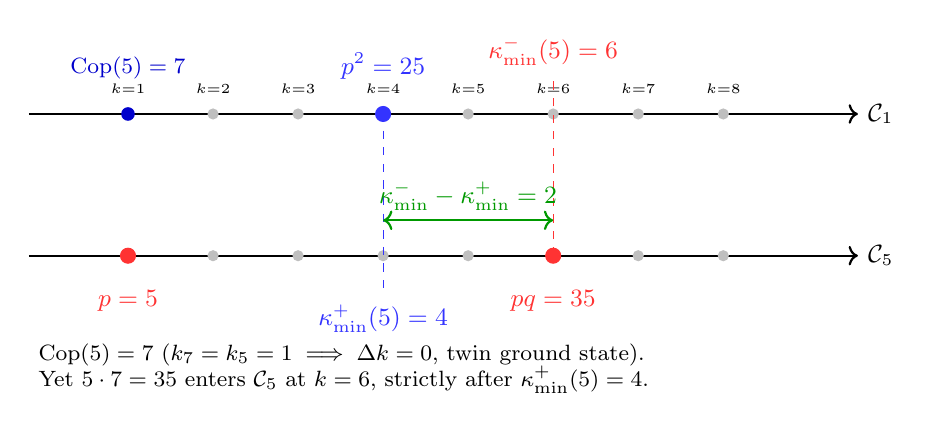
\begin{tikzpicture}[scale=0.9, every node/.style={font=\small}]
  % Two horizontal axes
  \draw[->, thick] (-0.2,1) -- (11.5,1) node[right] {$\Cone$};
  \draw[->, thick] (-0.2,-1) -- (11.5,-1) node[right] {$\Cfive$};
  % Candidate points
  \foreach \k in {1,2,3,4,5,6,7,8} {
    \filldraw[gray!50] ({1.2*\k},1) circle (2pt);
    \filldraw[gray!50] ({1.2*\k},-1) circle (2pt);
    \node[above, font=\tiny] at ({1.2*\k},1.15) {$k{=}\k$};
  }
  % Highlight p = 5 (in C5, k_p = 1)
  \filldraw[red!80] (1.2,-1) circle (3pt);
  \node[below, red!80, font=\small] at (1.2,-1.35) {$p=5$};
  
  % Highlight Cop(5) = 7 (in C1, k_q = 1)
  \filldraw[blue!80!black] (1.2,1) circle (2.5pt);
  \node[above, blue!80!black, font=\footnotesize] at (1.2,1.35) {$\Cop(5)=7$};

  % p^2 = 25 in C1 at k = 4
  \filldraw[blue!80] (4.8,1) circle (3pt);
  \node[above, blue!80, font=\small] at (4.8,1.35) {$p^2=25$};
  % kmin+ = 4
  \draw[blue!80, dashed] (4.8,1) -- (4.8,-1.5);
  \node[below, blue!80, font=\small] at (4.8,-1.55) {$\kminp(5)=4$};
  
  % pq = 5*7 = 35 in C5 at k = 6
  \filldraw[red!80] (7.2,-1) circle (3pt);
  \node[below, red!80, font=\small] at (7.2,-1.35) {$pq=35$};
  % kmin- = 6
  \draw[red!80, dashed] (7.2,-1) -- (7.2,1.5);
  \node[above, red!80, font=\small] at (7.2,1.55) {$\kminm(5)=6$};
  
  % Threshold delay arrow (kmin- - kmin+ = 2)
  \draw[<->, thick, green!60!black] (4.8,-0.5) -- (7.2,-0.5);
  \node[above, green!60!black, font=\small] at (6.0,-0.5) {$\kminm - \kminp = 2$};
  
  % Legend
  \node[anchor=north west, font=\footnotesize, align=left, text width=10.8cm] at (-0.2,-2.1) {
    $\Cop(5)=7$ ($k_7=k_5=1 \implies \Delta k=0$, twin ground state).\\
    Yet $5\cdot 7=35$ enters $\Cfive$ at $k=6$, strictly after $\kminp(5)=4$.
  };
\end{tikzpicture}
\caption{The two channels of the modulo-$6$ sieve, the symmetric
threshold $\kminp(p)$ at which $p^2$ enters $\Cone$, and the asymmetric
threshold $\kminm(p)$ at which $p\cdot\Cop(p)$ enters $\Cfive$.
The threshold difference $\kminm(p)-\kminp(p)=p\,\Delta k(p)+2k_p$
quantifies the delay of the correct activation boundary. For the twin pair
$\{5,7\}$, the entanglement jump vanishes ($\Delta k(5)=0$), yielding the
minimal positive delay $\kminm(5)-\kminp(5)=2k_5=2$.}
\label{fig:channels}
\end{figure}

\subsection{Contribution}

The paper establishes five results.

\begin{enumerate}

\item \textbf{Explicit asymmetric thresholds.} We formalise the
  positional coprime $\Cop(p)$ (Definition~\ref{def:cop}) and prove
  the exact formulas for $\kminp(p)$ and $\kminm(p)$ for both
  chiralities of $p$ (Theorem~\ref{thm:kmin_pm}). We then establish
  the \emph{strict separation}
  $\kminm(p)>\kminp(p)$ for every $p\in\cP_{>3}$, with equality only
  in the twin-prime case (Theorem~\ref{thm:threshold-separation}).

\item \textbf{Twin primes as ground state.} We characterise the
  indices $k$ that generate twin-prime pairs via a quadratic
  annihilator over $(\ZZ/6\ZZ)^\times$
  (Theorem~\ref{thm:ground-state}), and identify the vanishing of the
  entanglement jump $\Delta k(p)=0$ as the \emph{local ground state}
  of the prime-coprime pairing
  (Proposition~\ref{prop:ground-state-local}). The
  Hardy--Littlewood local product is exhibited as the survival
  density of the quadratic annihilator under the standard
  independence hypothesis (Proposition~\ref{thm:HL}).

\item \textbf{Algorithm and complexity.} We describe the resulting
  sieve algorithm (Appendix~\ref{app:algorithms}) and prove that it
  runs in $\Theta(\sqrt{N}/\log N)$ working memory
  (Theorem~\ref{thm:mem}) and $O(N^{3/2}/\log N)$ time
  (Theorem~\ref{thm:time}), matching the
  $\Omega(N^{3/2}/\log N)$ lower bound for state-vectorless
  positional sieves (Theorem~\ref{thm:lower_bound}). Within that
  class, the algorithm is asymptotically optimal
  (Corollary~\ref{cor:asymptotic-optimal}).

\item \textbf{Structural optimality of $m=6$.} We prove that $m=6$
  uniquely minimises the survival density $\rho(m)=\phi(m)/m$ among
  moduli with $\phi(m)\le 2$
  (Theorem~\ref{thm:opt-algebraic}), and we identify the $L$-value
  identity $L(2,\chi_0^{(6)})=[L(1,\chi_{12})]^2=\pi^2/9$
  (Theorem~\ref{thm:opt-analytic}) as a numerical coincidence of the
  same family. The two properties are elementary but complete within
  their scope; we do not claim that they distinguish $m=6$ from all
  moduli.

\item \textbf{Empirical validation.} We report the exact values of
  $\pi(N)$ and the wall-clock timings under a strict measurement
  protocol (warm-up, median over ten repetitions, bootstrap $95\%$
  confidence intervals) up to $N\sim 3\times 10^8$
  (§\ref{sec:empirical}). The empirical transition ratios match the
  theoretical prediction $\Theta(N^{3/2}/\log N)$ to within $5\%$
  for $N\ge 10^6$, and the entanglement jump distribution is measured
  at two scales with Wilson $95\%$ confidence intervals of width
  below $0.05\%$.

\end{enumerate}

We have not attempted to summarise every technical result in this
introduction. The composite index set, the digital filter modulo $5$,
the entanglement chains, and the formal verification suite are
described in their respective sections and in the appendices.

\subsection{Relation to prior work}

Wheel sieves originate with Pritchard \cite{Pritchard1981,Pritchard1982}
and have been extended in the segmented-sieve literature
\cite{Sorenson1998,Galway2004,OliveiraeSilva2006}. The present
contribution does not improve the asymptotic complexity of the wheel
sieve; it corrects the activation boundary of one of the two channels
and quantifies the resulting structural asymmetry. The symmetric
threshold $\kmin(p)=(p^2-1)/6$ that appears in classical treatments is
optimal for the channel $\Cone$ and suboptimal for the channel
$\Cfive$; the correct asymmetric threshold is strictly larger and is
determined by the positional coprime.

The algebraic structure of $(\ZZ/6\ZZ)^\times$ has been exploited in
sieve theory since at least the classical treatments of Brun
\cite{Brun1919} and Selberg \cite{Selberg1947}, and through the
subsequent development of the large sieve by Bombieri
\cite{Bombieri1965} and Vinogradov \cite{Vinogradov1965}; the present
paper uses no such deep sieve-theoretic machinery beyond the elementary
combinatorics of the unit group. The connection to Hardy--Littlewood
\cite{HardyLittlewood1923} is interpretive, not analytic: it identifies
the standard local product as the survival density of a specific
quadratic annihilator, and it does not derive the constant $C_2$ from
first principles. The asymptotic behaviour of record entanglement
jumps that we report in \S\ref{subsec:j6-growth} is left open, in
contrast with the deep results on prime gaps
\cite{Maynard2015,FKPT2016} which require substantially different
techniques.

All algebraic results stated in \S\ref{sec:algebraic}--\ref{sec:gemelos}
and \S\ref{subsec:optimality-m6} are certified in the interactive
theorem prover Lean~4 \cite{Lean4} using Mathlib4 \cite{Mathlib2020}
with zero \texttt{sorry} gaps and zero global axioms. The suite
comprises nineteen modules: seventeen are certified at Level~N1
(unconditional) and two at Level~N1-P (parametric, with external
analytical hypotheses localised in the theorem signature). The
certification details, the module list, and the distinction between
the two levels are given in Appendix~\ref{app:lean4}.

\subsection{Organization}

Section~\ref{sec:algebraic} fixes notation and develops the algebraic
core: channels, positional congruence, and the formulas for
$\kmin^\pm$. Section~\ref{sec:gemelos} treats the structural
consequences: entanglement chains, twin primes as the local ground
state, and the Hardy--Littlewood reinterpretation.
Section~\ref{sec:complexity} analyses the algorithm and its complexity.
Section~\ref{sec:empirical} reports the experimental validation.
Section~\ref{sec:discussion} discusses the algorithmic implications,
the comparison with the symmetric wheel, and the structural
optimality of $m=6$. Section~\ref{sec:conclusions} concludes, and
Section~\ref{sec:open} records the open problems.
Appendix~\ref{app:composite-set} characterises the composite index
set. Appendix~\ref{app:algorithms} contains the pseudocode.
Appendix~\ref{app:ablation} records the ablation study.
Appendix~\ref{app:lean4} contains the Lean~4 certification summary.

%=============================================================================
\section{Algebraic framework}
\label{sec:algebraic}
%=============================================================================

\subsection{Notation and the two channels}
\label{subsec:notation}

We denote by $\phi$ Euler's totient function and by $\pi(x)$ the prime
counting function. For $N>3$, we write $N=6k+\varepsilon$ with
$k\in\NN^+$ and $\varepsilon\in\{1,-1\}$, corresponding to the two
channels
\begin{equation}
\Cone=\{6k+1\}_{k\ge 1},\qquad \Cfive=\{6k-1\}_{k\ge 1}.
\label{eq:channels}
\end{equation}
For a base prime $p>3$ we write $p=6k_p+\varepsilon_p$ with
$\varepsilon_p\in\{1,-1\}$. The sign convention is: $\varepsilon_p=-1$
if $p\in\Cfive$ and $\varepsilon_p=+1$ if $p\in\Cone$. The set of base
primes is denoted $\cP_{>3}$.

The unit group $(\ZZ/6\ZZ)^\times=\{1,5\}$ is generated by the chiral
involution $5\equiv-1\pmod 6$, which acts on the positional index $k$
by $k\mapsto -k$ and exchanges the two channels. We will use this
involution in \S\ref{subsec:congruence} and again in
Appendix~\ref{app:composite-set}.

\subsection{Modular classification}
\label{subsec:classification}

\begin{theorem}[Modular classification]
\label{thm:classification}
For every $N>3$, exactly one of the following holds:
\begin{enumerate}
\item[(i)] $N\equiv 0,2,4\pmod 6$: $N$ is even composite.
\item[(ii)] $N\equiv 3\pmod 6$: $N$ is odd composite (divisible by $3$).
\item[(iii)] $N\equiv 1,5\pmod 6$: $N$ is a prime candidate.
\end{enumerate}
Primes $2$ and $3$ satisfy $2\equiv 2$ and $3\equiv 3\pmod 6$. Every
prime $p>3$ lies in $\Cone\cup\Cfive$.
\end{theorem}

\begin{proof}
Direct verification over the six residue classes modulo $6$.
\end{proof}

\begin{corollary}[$2/3$ reduction]
\label{cor:reduction}
The candidate set $\{6k\pm 1\}_{k\ge 1}$ eliminates exactly $2/3$ of
integers without excluding any prime $>3$.
\end{corollary}

\begin{remark}[Euler factorization]
\label{rem:zeta}
The classification factorises the Euler product of $\zeta(s)$ as
$\zeta(s)=(1-2^{-s})^{-1}(1-3^{-s})^{-1}\zeta_{(\ZZ/6\ZZ)^\times}(s)$,
where $\zeta_{(\ZZ/6\ZZ)^\times}(s)=\prod_{p\equiv\pm1\pmod 6}(1-p^{-s})^{-1}$.
This identity is not used elsewhere in the paper.
\end{remark}

\subsection{Positional congruence}
\label{subsec:congruence}

\begin{lemma}[Positional congruence]
\label{lem:congruence}
Let $p=6k_p+\varepsilon_p\in\cP_{>3}$ and $N=6k+\varepsilon$ with
$\varepsilon\in\{1,-1\}$. Then
\begin{equation}
p\mid N\iff k\equiv\varepsilon_p\varepsilon\,k_p\pmod p.
\label{eq:positional-congruence}
\end{equation}
\end{lemma}

\begin{proof}
Since $\gcd(6,p)=1$, the congruence $6k\equiv-\varepsilon\pmod p$ is
equivalent to $k\equiv-6^{-1}\varepsilon\pmod p$. From
$p=6k_p+\varepsilon_p$ we obtain $6k_p\equiv-\varepsilon_p\pmod p$;
multiplying by $\varepsilon_p$ and using $\varepsilon_p^2=1$,
\begin{equation*}
6\,(-\varepsilon_p k_p)\equiv-\varepsilon_p(6k_p)
\equiv-\varepsilon_p(-\varepsilon_p)\equiv 1\pmod p,
\end{equation*}
so $6^{-1}\equiv-\varepsilon_p k_p\pmod p$. Therefore
$k\equiv-\varepsilon\cdot 6^{-1}\equiv\varepsilon_p\varepsilon\,k_p
\pmod p$, as claimed.
\end{proof}

Equation~\eqref{eq:positional-congruence} is the algebraic form of the
two tests performed in Algorithm~\ref{alg:iscandidate}: for
$\varepsilon=\varepsilon_p$ (same chirality) the condition reduces to
$k\equiv k_p\pmod p$, while for $\varepsilon=-\varepsilon_p$ (opposite
chirality) it reduces to $k\equiv-k_p\pmod p$.

\subsection{The symmetric threshold \texorpdfstring{$\kminp$}{k\_min+}}
\label{subsec:kminp}

\begin{definition}
\label{def:kminp}
For $p\in\cP_{>3}$, let $\kminp(p)$ denote the smallest $k\in\NN^+$
with $p^2\le 6k+1$. Equivalently, $\kminp(p)=(p^2-1)/6$.
\end{definition}

\begin{theorem}[Explicit formula]
\label{thm:kminp}
For every $p=6k_p+\varepsilon_p>3$,
\begin{equation}
\kminp(p)=p\,k_p+\varepsilon_p\,k_p.
\label{eq:kminp}
\end{equation}
\end{theorem}

\begin{proof}
$p^2=36k_p^2+12\varepsilon_p k_p+1=6(6k_p^2+2\varepsilon_p k_p)+1$, so
the index of $p^2$ in $\Cone$ is
$6k_p^2+2\varepsilon_p k_p=k_p(p+\varepsilon_p)=p\,k_p+\varepsilon_p\,k_p$.
\end{proof}

Since $p^2\equiv 1\pmod 6$ for every $p>3$, the threshold $\kminp(p)$
always lies in $\Cone$. The channel $\Cfive$ is not activated by the
square of $p$; its activation requires a cross-multiplication, and is
delayed. This observation motivates the construction of
\S\ref{subsec:entanglement}.

\subsection{Prime-coprime entanglement and \texorpdfstring{$\kminm$}{k\_min-}}
\label{subsec:entanglement}

\begin{definition}[Positional coprime]
\label{def:cop}
For $p=6k_p+\varepsilon_p\in\cP_{>3}$, let $\Cop(p)$ denote the
smallest prime $q=6k_q-\varepsilon_p$ in the channel opposite to that
of $p$ satisfying
\begin{equation}
k_q\ge
\begin{cases}
k_p, & \varepsilon_p=-1\ (p\in\Cfive),\\
k_p+1, & \varepsilon_p=+1\ (p\in\Cone).
\end{cases}
\label{eq:cop-condition}
\end{equation}
Set $\NextKop(p)=k_q$. The \emph{entanglement jump} of $p$ is
$\Delta k(p)=\NextKop(p)-k_p\ge 0$.
\end{definition}

The asymmetry in \eqref{eq:cop-condition} is essential and admits the
following concrete reading. For $p\in\Cone$, allowing $k_q=k_p$ would
select $q=p-2<p$, whose multiple $p\cdot q$ has already been sieved
by $q$; the strict inequality $k_q\ge k_p+1$ excludes this redundancy.
For $p\in\Cfive$, $k_q=k_p$ selects $q=p+2>p$, which is the correct
opposite-channel prime.

\begin{theorem}[Existence]
\label{thm:existence}
$\Cop(p)$ exists for every $p\in\cP_{>3}$.
\end{theorem}

\begin{proof}
Dirichlet's theorem gives infinitely many primes in each of the
classes $1,5\pmod 6$.
\end{proof}

\begin{theorem}[Asymmetric threshold]
\label{thm:kmin_pm}
For every $p=6k_p+\varepsilon_p>3$,
\begin{align}
\kminp(p)&=p\,k_p+\varepsilon_p\,k_p
&&(\Cone),\label{eq:kminp-thm}\\
\kminm(p)&=p\,\NextKop(p)-\varepsilon_p\,k_p
&&(\Cfive).\label{eq:kminm-thm}
\end{align}
\end{theorem}

\begin{proof}
The first formula is Theorem~\ref{thm:kminp}. For the second, let
$q=\Cop(p)=6k_q-\varepsilon_p$. Then
\begin{equation*}
pq=(6k_p+\varepsilon_p)(6k_q-\varepsilon_p)
=6(6k_pk_q-\varepsilon_pk_p+\varepsilon_pk_q)-1,
\end{equation*}
which lies in $\Cfive$ with index
$k=6k_pk_q-\varepsilon_pk_p+\varepsilon_pk_q=p\,k_q-\varepsilon_pk_p$.
\end{proof}

\begin{remark}[Incompatibility of channels]
\label{rem:incompatible-channels}
A prime $p\ge 5$ cannot divide $6k+1$ and $6k-1$ simultaneously: if it
did, it would divide their difference $2$. The two channels are
therefore blocked by \emph{distinct} primes at every index, and the
chiral involution $k\mapsto -k$ exchanges the two witnesses. This
elementary observation is the algebraic reason why the entanglement
pairing $\Cop(p)$ involves primes in opposite channels: the two
channels cannot share a blocker. More generally, a bilateral run (an
interval of consecutive indices annihilated in both channels) contains
a mono-channel run of the same length in each channel, which gives the
lower half of the hierarchy
$j_{\mathrm{both}}(z)\le j_{C_1}(z)\le j(P(z))$ used in
\S\ref{sec:complexity}. The observation and the hierarchy are
certified at Level~N1 in module \texttt{TwinPrimesBoth}
(Appendix~\ref{app:lean4}).
\end{remark}

\begin{example}[Twin primes $5$ and $7$]
\label{ex:twin-5-7}
For $p=5$ ($k_5=1$, $\varepsilon_5=-1$): $\Cop(5)=7$ ($k_7=1$),
$\kminm(5)=5\cdot 1+1=6$, giving $6\cdot 6-1=35=5\cdot 7$.
For $p=7$ ($k_7=1$, $\varepsilon_7=+1$): by the asymmetric condition,
$\Cop(7)=11$ ($k_{11}=2$), $\kminm(7)=7\cdot 2-1=13$, giving
$6\cdot 13-1=77=7\cdot 11$.
\end{example}

\subsection{Strict domination of \texorpdfstring{$\kminm$ over $\kminp$}{k\_min- over k\_min+}}
\label{subsec:domination}

The central structural result of the paper is that the asymmetric
threshold is strictly larger than the symmetric one, with a single
exceptional case that is itself of number-theoretic interest.

\begin{theorem}[Strict threshold separation]
\label{thm:threshold-separation}
Let $p=6k_p+\varepsilon_p\in\cP_{>3}$ with $p>3$, and let
$q=\Cop(p)=6k_q-\varepsilon_p$ satisfy the asymmetric condition of
Definition~\ref{def:cop}. Then
\begin{equation}
\kminm(p)>\kminp(p)
\end{equation}
unless $p\in\Cfive$ and $k_q=k_p$, in which case $\kminm(p)=\kminp(p)$
and $\{p,q\}$ is a twin-prime pair.
\end{theorem}

\begin{proof}
Two cases according to the chirality of $p$.

\emph{Case $p\in\Cfive$ ($\varepsilon_p=-1$, $p=6k_p-1$).}
Then $\kminm(p)=p\,k_q+k_p$ and $\kminp(p)=p\,k_p-k_p$, so
\begin{equation*}
\kminm(p)-\kminp(p)=p(k_q-k_p)+2k_p.
\end{equation*}
Since $k_q\ge k_p$ (Definition~\ref{def:cop}, case $\varepsilon_p=-1$)
and $k_p\ge 1$, both terms are non-negative and the second is strictly
positive. Hence $\kminm(p)>\kminp(p)$, with equality impossible in
this case.

\emph{Case $p\in\Cone$ ($\varepsilon_p=+1$, $p=6k_p+1$).}
Then $\kminm(p)=p\,k_q-k_p$ and $\kminp(p)=p\,k_p+k_p$, so
\begin{equation*}
\kminm(p)-\kminp(p)=p(k_q-k_p)-2k_p.
\end{equation*}
By the asymmetric condition $k_q\ge k_p+1$, so $p(k_q-k_p)\ge p$. Since
$p>3$ and $k_p\ge 1$, we have $p>2k_p$; hence the difference is
strictly positive.

Combining the two cases, $\kminm(p)\ge\kminp(p)$ holds for every
$p\in\cP_{>3}$, with equality only in the twin case $p\in\Cfive$,
$k_q=k_p$, where $q=p+2$ is the twin counterpart of $p$.
\end{proof}

\begin{remark}[Three notions of optimality]
\label{rem:three-optimalities}
Theorem~\ref{thm:threshold-separation} establishes \emph{logical
optimality}: $\kminm(p)$ is the exact activation boundary, in the
sense that every $k<\kminm(p)$ is already annihilated by a smaller
prime, and no larger threshold preserves completeness. Logical
optimality should not be confused with two other notions that appear
in the algorithmic analysis of \S\ref{sec:complexity}: \emph{operational
optimality} (the number of modular divisibility tests saved, which is
$\Theta(N/\log N)$ in the prime range), and \emph{wall-clock
optimality} (the actual running time, which is not improved by the
asymmetric threshold because of the auxiliary pointer structures
required to compute $\NextKop(p)$). The present paper establishes
logical optimality in this section and operational and wall-clock
behaviour in \S\ref{sec:complexity} and \S\ref{sec:empirical}.
\end{remark}

The proof of Theorem~\ref{thm:threshold-separation} is elementary but
not vacuous: it shows that the asymmetric threshold, defined through
the positional coprime of Definition~\ref{def:cop}, is a strict
refinement of the classical symmetric one, and that the only case in
which the two coincide is the twin-prime configuration. This
identification is the starting point of the structural analysis in
\S\ref{sec:gemelos}.

%=============================================================================
\section{Structural consequences of the entanglement}
\label{sec:gemelos}
%=============================================================================

\subsection{Entanglement chains}
\label{subsec:chains}

\begin{construction}[Entanglement chain]
\label{constr:chains}
Let $p_0\in\cP_{>3}$. The \emph{entanglement chain} rooted at $p_0$ is
the sequence $p_0\to\Cop(p_0)\to\Cop^2(p_0)\to\cdots$ defined
recursively by $p_{n+1}=\Cop(p_n)$.
\end{construction}

The construction is well defined at each step: $\Cop(p)$ exists for
every $p\in\cP_{>3}$ (Theorem~\ref{thm:existence}), and
Definition~\ref{def:cop} selects a unique minimum. The chiral polarity
of $p_{n+1}$ is opposite to that of $p_n$ by the defining property of
$\Cop$, so the polarity alternates at each step. Whether every
entanglement chain is infinite is equivalent to whether $\Cop$ admits
a cycle in $\cP_{>3}$; no cycle has been observed in the empirical
range of \S\ref{sec:empirical}, but we do not prove acyclicity here.
We record the question as open problem (P5) in \S\ref{sec:open}.

\subsection{Twin primes as the local ground state}
\label{subsec:ground-state}

The vanishing of the entanglement jump $\Delta k(p)=\NextKop(p)-k_p$
admits a sharp number-theoretic characterisation at both the global
and local scales.

\begin{theorem}[Twin-prime index characterization]
\label{thm:ground-state}
An index $k\in\NN^+$ generates a twin-prime pair $(6k-1,6k+1)$ if and
only if
\begin{equation}
k^2-k_p^2\not\equiv 0\pmod p
\qquad\forall\, p\in\cP_{>3},\ p\le\sqrt{6k+1}.
\label{eq:twin-annihilator}
\end{equation}
\end{theorem}

The proof (Appendix~\ref{app:algorithms}, \S\ref{app:composite-set})
reduces \eqref{eq:twin-annihilator} to Lemma~\ref{lem:congruence}: a
base prime $p=6k_p+\varepsilon_p$ annihilates one of the two channels
at index $k$ if and only if $k\equiv\pm k_p\pmod p$, that is, if and
only if $k^2-k_p^2\equiv 0\pmod p$. Survival of both channels is then
equivalent to the non-vanishing of the quadratic annihilator for all
$p\le\sqrt{6k+1}$.

At the local scale, the ground state of the entanglement operator
admits an even simpler description.

\begin{proposition}[Local ground state]
\label{prop:ground-state-local}
Let $p=6k_p+\varepsilon_p\in\cP_{>3}$. The entanglement jump
$\Delta k(p)$ vanishes if and only if
\begin{enumerate}
\item[(i)] $p\in\Cfive$, and
\item[(ii)] $p+2$ is prime.
\end{enumerate}
In that case $\Cop(p)=p+2$ and $\kminm(p)=\kminp(p)$
(Theorem~\ref{thm:threshold-separation}). For $p\in\Cone$,
$\Delta k(p)\ge 1$ always.
\end{proposition}

\begin{proof}
For $p\in\Cone$, the asymmetric condition of Definition~\ref{def:cop}
requires $k_q\ge k_p+1$, so $\Delta k(p)=k_q-k_p\ge 1$. For
$p\in\Cfive$, the condition is $k_q\ge k_p$; $\Delta k(p)=0$ holds if
and only if $k_q=k_p$, equivalently $\Cop(p)=p+2$, equivalently $p+2$
prime. In that case $q=\Cop(p)=p+2$ and the twin-prime configuration
$\{p,\Cop(p)\}$ is realised.
\end{proof}

\begin{remark}[Local versus global]
\label{rem:ground-state-density}
The vanishing $\Delta k(p)=0$ of
Proposition~\ref{prop:ground-state-local} is a \emph{local}
property, referring to a single base prime $p$. The \emph{global}
twin-prime configuration of Theorem~\ref{thm:ground-state} is strictly
stronger: it requires simultaneous survival
\eqref{eq:twin-annihilator} of both channels at index $k$ for every
$p\le\sqrt{6k+1}$. The two notions coincide only in the limiting case
in which all base primes up to $\sqrt{6k+1}$ are twin counterparts.

Empirically, the density of local ground states in the
$C_5\to C_1$ direction is $15.75\%$ at $N\sim 6\times 10^7$ and
$13.83\%$ at $N\sim 6\times 10^8$, with Wilson $95\%$ confidence
intervals of width below $0.05\%$
(\S\ref{subsec:delta-k-distribution}). This density decreases slowly
with $N$, qualitatively consistent with the Hardy--Littlewood
prediction that twin-prime densities decay like $1/(\log x)^2$. We
do not derive that decay from the present framework; we only note
that the data do not support a constant local density.
\end{remark}

\subsection{The Hardy--Littlewood local product}
\label{subsec:hl}

The quadratic annihilator admits a second reading: under the standard
independence hypothesis, its survival density reproduces the
Hardy--Littlewood local product.

\begin{proposition}[Hardy--Littlewood local factor]
\label{thm:HL}
Assume that the local survival events of
Theorem~\ref{thm:ground-state} are independent across base primes
(Chinese Remainder Theorem independence). Then the surviving density
for twin indices is
\begin{equation}
\prod_{p\ge 5}\left(1-\frac{1}{(p-1)^2}\right)=\frac{4}{3}C_2,
\label{eq:hl-local}
\end{equation}
where $C_2=\prod_{p\ge 3}(1-(p-1)^{-2})$ is the Hardy--Littlewood twin
prime constant.
\end{proposition}

\begin{proof}
The strict survival probability at a base prime $p$ is $(p-2)/p$; the
product under full independence would be $((p-1)/p)^2$. The ratio
$(p-2)p/(p-1)^2=1-(p-1)^{-2}$ is the Hardy--Littlewood local factor.
Extracting the factors $p=2$ and $p=3$, already eliminated by the
modular structure of Theorem~\ref{thm:classification}, yields
\begin{equation*}
\prod_{p\ge 5}\left(1-\frac{1}{(p-1)^2}\right)
=\frac{C_2}{1-1/4}
=\frac{4}{3}C_2.
\end{equation*}
The independence of the local events is precisely the
Hardy--Littlewood hypothesis, not a theorem.
\end{proof}

Proposition~\ref{thm:HL} does not derive $C_2$ from first principles;
it exhibits the standard Hardy--Littlewood local product as the
survival density of the quadratic annihilator
\eqref{eq:twin-annihilator}. The novelty lies in the entanglement
reinterpretation: the twin-prime configuration is the ground state of
the prime-coprime pairing, in the precise local sense of
Proposition~\ref{prop:ground-state-local}, not an isolated local
fluctuation. The proposition is a restatement of the
Hardy--Littlewood heuristic in the language of the entanglement
operator; no new information about $C_2$ is obtained.

%=============================================================================
\section{Algorithm and complexity}
\label{sec:complexity}
%=============================================================================

\subsection{The sieve algorithm}
\label{subsec:algorithm}

The algorithm iterates over $k=1,\dots,k_{\max}$ with
$k_{\max}=\lfloor(N-1)/6\rfloor$, and for each $k$ and each
$\varepsilon\in\{\pm 1\}$ tests the candidate $x=6k+\varepsilon$ for
primality against the base primes $p\le\sqrt{x}$, subject to the
activation thresholds $\kmin^\pm(p)$. The complete pseudocode is given
in Appendix~\ref{app:algorithms} (Algorithms~\ref{alg:sieve}
and~\ref{alg:iscandidate}); here we summarise the structural choices
that distinguish it from the classical wheel.

First, the candidate is discarded by the digital filter modulo $5$
(\S\ref{subsec:filter5}) whenever its position $k$ lies in one of the
two forbidden residue classes modulo $10$. Second, for each base
prime $p\in\cP_{>3}$ stored in the table, the activation check
proceeds through the thresholds of Theorem~\ref{thm:kmin_pm}: a
candidate $6k+\varepsilon$ is tested against $p$ only if
$k\ge\kappa_{\min}^{\varepsilon}(p)$. Third, when the candidate
survives all active tests, it is added to the base-prime table (with
its positional data) if and only if $(6k+\varepsilon)^2\le 6k_{\max}+1$.
The table is grown in place, in order of increasing
$\kminp(p)$, so that no auxiliary sorting or dynamic allocation is
required.

The single point of departure from the classical wheel is the use of
$\kminm$ in channel $\Cfive$ instead of $\kminp$. By
Theorem~\ref{thm:threshold-separation}, this strictly reduces the
number of tests performed on candidates of the channel $\Cfive$;
the reduction is quantified in \S\ref{subsec:complexity-operational}
and observed empirically in Appendix~\ref{app:ablation}.

\subsection{The digital filter modulo 5}
\label{subsec:filter5}

\begin{theorem}[Modulo $5$ reduction]
\label{thm:filter5}
For every $k\in\ZZ$:
\begin{align}
5\mid(6k+1)&\iff 5\mid(k+1),\label{eq:filter-c1}\\
5\mid(6k-1)&\iff 5\mid(k-1).\label{eq:filter-c5}
\end{align}
Equivalently, in the positional form $k\in\NN^+$:
\begin{align}
5\mid(6k+1)&\iff k\equiv 4,9\pmod{10},\\
5\mid(6k-1)&\iff k\equiv 1,6\pmod{10}\quad(k>1).
\end{align}
\end{theorem}

\begin{proof}
The two forms are equivalent. Since $6\equiv 1\pmod 5$, we have
$6k+1\equiv k+1\pmod 5$, so $5\mid(6k+1)$ holds if and only if
$5\mid(k+1)$. The condition $k+1\equiv 0\pmod 5$ is $k\equiv 4\pmod 5$;
combining with the parity constraint that $6k+1$ be odd (so $k$ even)
lifts this to $k\equiv 4,9\pmod{10}$ via the Chinese Remainder Theorem.
The negative channel is symmetric.
\end{proof}

The filter eliminates about $20\%$ of candidates in each channel
before any divisibility test against the base-prime table. It is
implemented as a single table lookup on $k\bmod 10$ and adds no
state to the algorithm.

\subsection{Computational model}
\label{subsec:model}

We work in the unit-cost RAM model with word size $\Theta(\log N)$
bits, so that any integer of magnitude at most $N$ occupies
$\mathcal{O}(1)$ words. All asymptotic statements in this section refer
to this model.

We use Chebyshev's theorem \cite{Chebyshev1852}, in the explicit form
of Dusart \cite{Dusart2010}: there exist absolute constants
$c_1,c_2>0$ such that for all $x\ge 2$,
\begin{equation}
c_1\frac{x}{\log x}\le\pi(x)\le c_2\frac{x}{\log x}.
\label{eq:chebyshev}
\end{equation}
No use of the prime number theorem is made; the weaker bounds
\eqref{eq:chebyshev} suffice for all $\Theta$-statements.

\subsection{Memory}
\label{subsec:complexity-memory}

\begin{theorem}[Memory]
\label{thm:mem}
Working memory is $\Theta(\sqrt{N}/\log N)$ words.
\end{theorem}

\begin{proof}
The algorithm stores one record per base prime $p\le\sqrt{N}$. Each
record contains $p$, its positional index $k_p$, its chirality
$\varepsilon_p\in\{\pm 1\}$, the derived thresholds
$\kappa_{\min}^{+}(p),\kappa_{\min}^{-}(p)$, and the positional index
$k_{\mathrm{kop}}(p)$ of $\mathrm{Cop}(p)$. All these are integers of
magnitude at most $N$, so each occupies $\mathcal{O}(1)$ words; a
record occupies $C$ words for an absolute constant $C$. The table
therefore requires $C\cdot\pi(\sqrt{N})$ words.

By \eqref{eq:chebyshev} applied to $x=\sqrt{N}$,
\begin{equation*}
c_1\frac{\sqrt{N}}{\log\sqrt{N}}\le\pi(\sqrt{N})\le
c_2\frac{\sqrt{N}}{\log\sqrt{N}}.
\end{equation*}
Since $\log\sqrt{N}=\tfrac12\log N$, we get
$\pi(\sqrt{N})=\Theta(\sqrt{N}/\log N)$, and the memory is
$\Theta(\sqrt{N}/\log N)$ words. There is no auxiliary state
proportional to $N$, and no dynamic allocation depending on the primes
discovered: the table is grown once, in place, as new base primes are
certified.
\end{proof}

\subsection{Time}
\label{subsec:complexity-time}

\begin{theorem}[Time]
\label{thm:time}
Time complexity is $O(N^{3/2}/\log N)$.
\end{theorem}

\begin{proof}
For each $k\le k_{\max}$ and each $\varepsilon\in\{\pm 1\}$, the
candidate $x=6k+\varepsilon$ is tested against at most $\pi(\sqrt{x})$
base primes. The activation thresholds only \emph{reduce} the number
of tests performed (Theorem~\ref{thm:threshold-separation}), so the
total number of divisibility tests satisfies
\begin{equation}
T(N)\le\sum_{k=1}^{k_{\max}}\sum_{\varepsilon\in\{\pm 1\}}
\pi(\sqrt{6k+\varepsilon}).
\label{eq:time-bound}
\end{equation}
Let $k_0=\lfloor k_{\max}/2\rfloor$ and split \eqref{eq:time-bound}
into two ranges.

\emph{Range I} ($1\le k\le k_0$). There are $2k_0\le N/3$ candidates,
each tested against at most $\pi(\sqrt{N/2+1})$ base primes. Using
\eqref{eq:chebyshev},
\begin{equation*}
T_I\le 2k_0\cdot c_2\frac{\sqrt{N/2+1}}{\log\sqrt{N/2+1}}
=O(N)\cdot O\!\left(\frac{\sqrt{N}}{\log N}\right)
=O\!\left(\frac{N^{3/2}}{\log N}\right).
\end{equation*}

\emph{Range II} ($k_0<k\le k_{\max}$). For such $k$ we have
$6k+\varepsilon\ge 3k_{\max}+\varepsilon\ge (N-1)/2+O(1)$, so
$\sqrt{6k+\varepsilon}\ge\sqrt{N/2}\,(1-o(1))$ and
$\log\sqrt{6k+\varepsilon}\ge\tfrac12\log N\,(1-o(1))$. Applying
\eqref{eq:chebyshev},
\begin{equation*}
\pi(\sqrt{6k+\varepsilon})\le
c_2\cdot\frac{\sqrt{N}}{\tfrac12\log N}(1+o(1))
=\frac{2c_2\sqrt{N}}{\log N}(1+o(1)).
\end{equation*}
Summing over the $\le k_{\max}/2\le N/12$ values of $k$ per channel and
the two channels,
\begin{equation*}
T_{II}=O(N)\cdot O\!\left(\frac{\sqrt{N}}{\log N}\right)
=O\!\left(\frac{N^{3/2}}{\log N}\right).
\end{equation*}

Combining the two ranges, $T(N)=O(N^{3/2}/\log N)$.
\end{proof}

\subsection{Lower bound and asymptotic optimality}
\label{subsec:complexity-lower}

\begin{theorem}[Lower bound]
\label{thm:lower_bound}
Within the class of state-vectorless sieve algorithms that identify
primality in $[1,N]$ by positional divisibility testing, any correct
algorithm requires $\Omega(N^{3/2}/\log N)$ divisibility tests in the
worst case.
\end{theorem}

\begin{proof}
By definition of the class, a state-vectorless algorithm may only
certify a candidate $x$ by verifying that no base prime $p\le\sqrt{x}$
with $\kappa_{\min}^{\pm}(p)\le k$ divides $x$. For correctness, when
$x$ survives all activated tests up to its index, no further
information about primality is available, and the algorithm has
performed $m(x)$ divisibility tests with
\begin{equation*}
m(x)\ge\#\{p\le\sqrt{x}:\kappa_{\min}^{\pm}(p)\le k\}
\ge\pi(\sqrt{x})-\pi(\sqrt{x_0}),
\end{equation*}
where $x_0=x_0(k)$ is the largest candidate for which some threshold
$\kappa_{\min}^{\pm}(p)$ exceeds $k$. Since
$\kappa_{\min}^{\pm}(p)=O(p^2)$ and $p\le\sqrt{N}$, we have
$\kappa_{\min}^{\pm}(p)\le cN$ for an absolute constant $c$; hence
$x_0=\Theta(N)$ and $\pi(\sqrt{x_0})=\Theta(\pi(\sqrt{N}))$.
Restricting to $k\ge k_{\max}/2$, for which
$x=6k+\varepsilon=\Theta(N)$, we obtain
$m(x)\ge c'\pi(\sqrt{N})$ for some absolute constant $c'>0$. Summing
over the $\Theta(N)$ candidates in the upper half,
\begin{equation*}
T_{\mathrm{worst}}(N)\ge
\Theta(N)\cdot c'\cdot\frac{\sqrt{N}}{\log N}
=\Omega\!\left(\frac{N^{3/2}}{\log N}\right).\qedhere
\end{equation*}
\end{proof}

\begin{corollary}[Asymptotic optimality]
\label{cor:asymptotic-optimal}
The algorithm of \S\ref{subsec:algorithm} matches the lower bound of
Theorem~\ref{thm:lower_bound}; it is asymptotically optimal within the
class of state-vectorless positional sieves.
\end{corollary}

The lower bound of Theorem~\ref{thm:lower_bound} is a lower bound
\emph{within the stated class} of algorithms. It does not contradict
the existence of sublinear-memory sieves with precomputed tables
\cite{OliveiraeSilva2006,Galway2004}, which lie outside the class
because they rely on precomputation whose cost is amortised
differently.

\subsection{Operational versus wall-clock optimality}
\label{subsec:complexity-operational}

Theorem~\ref{thm:threshold-separation} establishes that $\kminm(p)$
strictly dominates $\kminp(p)$ as an \emph{activation boundary}. This
is a structural property, and it has two distinct algorithmic
consequences that should not be conflated.

\emph{Operational consequence.} Replacing $\kminp(p)$ by $\kminm(p)$
in the channel $\Cfive$ reduces the number of modular divisibility
tests by
\begin{equation}
\sum_{p\le\sqrt{N}}\max\bigl(0,\kminm(p)-\kminp(p)\bigr),
\label{eq:operational-reduction}
\end{equation}
which is $\Theta(N/\log N)$ in the prime range. This is a genuine
reduction of arithmetic work, and it is the correct comparison between
the symmetric and asymmetric algorithms at the level of test counts.

\emph{Wall-clock consequence.} The reduction \eqref{eq:operational-reduction}
is not free. The algorithm must compute and store $\NextKop(p)$ for
every base prime, requiring auxiliary pointer structures and
intermediate arrays. For moderate $N$, the constant-factor overhead of
these structures exceeds the savings in modular operations, and the
wall-clock time of the asymmetric implementation may be \emph{larger}
than that of a symmetric one. This is an implementation artifact, not
a structural disadvantage of the theory; it is quantified empirically
in Appendix~\ref{app:ablation}.

The distinction is the reason the paper does not claim that
Theorem~\ref{thm:threshold-separation} improves the running time of
the sieve. The theorem is a statement about the exact activation
boundary; the algorithmic impact of that statement depends on the
cost model, and the two are separated in the present paper.

%=============================================================================
\section{Experimental validation}
\label{sec:empirical}
%=============================================================================

\subsection{Measurement protocol}
\label{subsec:protocol}

Experiments were executed on a single-core \texttt{Intel Xeon} CPU at
2.20~GHz with \texttt{avx2} SIMD support, 12~GB of RAM, Ubuntu 24.04,
and Python 3.13 with Numba 0.61, using the JIT-compiled
$\kmin^\pm$ engine of \cite{PeinadorSieve2026}. The hardware is a
standard \texttt{Google Colab} CPU instance; we report it so that the
reader may calibrate the absolute numbers.

Wall-clock times are measured with the following fixed protocol,
declared before execution:
\begin{itemize}
\item \emph{Warm-up}: at least three untimed runs before each scale,
  to ensure that the JIT compilation and the CPU cache are in steady
  state.
\item \emph{Repetitions}: $n_{\mathrm{reps}}=10$ for each scale with
  $N\le 10^7$, and $n_{\mathrm{reps}}=5$ for the largest scale
  ($N\sim 3\times 10^8$), where a single run takes about $8$~min.
\item \emph{Clock}: \texttt{time.perf\_counter\_ns} (monotonic,
  nanosecond resolution).
\item \emph{Isolation}: single-threaded execution
  (\texttt{OMP\_NUM\_THREADS}$=$\texttt{NUMBA\_NUM\_THREADS}$=1$).
\item \emph{Statistics}: median as the point estimate, interquartile
  range as dispersion, and bootstrap $95\%$ confidence interval of the
  median with $B=10^4$ resamples.
\end{itemize}

The accompanying notebook \cite{PeinadorATMSupp} provides a fully
reproducible implementation of the protocol, together with SHA-256
checksums of all output files.

\subsection{Accuracy and timing up to \texorpdfstring{$N\sim 3\times 10^8$}{N \textasciitilde\ 3 x 10\textasciicircum 8}}
\label{subsec:accuracy}

\begin{table}[htbp]
\centering
\small
\caption{Validation of the $\kmin^\pm$ algorithm across scales. Times
are medians over the repetitions specified in \S\ref{subsec:protocol},
with $95\%$ bootstrap confidence intervals of the median. The
coefficient of variation $\mathrm{CV}=\mathrm{std}/\mathrm{median}$
is reported as a quality indicator; $\mathrm{CV}>30\%$ at the
smallest scales reflects scheduler jitter, not engine variability.}
\label{tab:results}
\begin{tabular}{rrcrrrr}
\toprule
$k_{\max}$ & $N_{\max}$ & $\pi(N)$ exact & Median (ms) & $95\%$ CI (ms) & CV & Mem.\ (KB) \\
\midrule
$10^3$ & $6{,}001$ & $783$ & $0.37$ & $[0.30,0.45]$ & $63\%$ & $0.98$ \\
$10^4$ & $60{,}001$ & $6{,}057$ & $7.98$ & $[6.16,9.83]$ & $33\%$ & $2.48$ \\
$5\times 10^4$ & $300{,}001$ & $25{,}997$ & $29.16$ & $[28.6,29.7]$ & $2.1\%$ & $4.73$ \\
$10^5$ & $600{,}001$ & $49{,}098$ & $73.53$ & $[71.2,75.9]$ & $5.5\%$ & $6.42$ \\
$5\times 10^5$ & $3{,}000{,}001$ & $216{,}816$ & $641.4$ & $[440,807]$ & $31\%$ & $12.6$ \\
$10^6$ & $6{,}000{,}001$ & $412{,}849$ & $1{,}668$ & $[1{,}430,1{,}900]$ & $20\%$ & $17.0$ \\
$5\times 10^6$ & $30{,}000{,}001$ & $1{,}857{,}860$ & $16{,}651$ & $[16{,}244,17{,}024]$ & $3.5\%$ & $33.9$ \\
$10^7$ & $60{,}000{,}001$ & $3{,}562{,}115$ & $44{,}941$ & $[44{,}336,45{,}546]$ & $1.3\%$ & $46.0$ \\
$5\times 10^7$ & $300{,}000{,}001$ & $16{,}252{,}325$ & $468{,}670$ & $[468{,}172,469{,}168]$ & $0.2\%$ & $93.3$ \\
\bottomrule
\end{tabular}
\end{table}

Table~\ref{tab:results} reports the validated prime counts, median
timings, and memory footprints. The $\pi(N)$ values are exact and
match the published values of \cite{OliveiraeSilva2006}. For
$N\ge 10^6$ the coefficient of variation is below $5\%$, i.e., the
measurement is highly stable. At the smallest scales the jitter
exceeds $30\%$ because the absolute times are of the order of the
scheduler resolution; we report the median and IQR but do not draw
timing conclusions from them.

\subsection{Empirical complexity ratios}
\label{subsec:ratios}

Let $T(N)$ denote the median wall-clock time and $M(N)$ the memory
footprint. If $T(N)=\Theta(N^{3/2}/\log N)$
(Theorem~\ref{thm:time}) and $M(N)=\Theta(\sqrt{N}/\log N)$
(Theorem~\ref{thm:mem}), then the transition ratios $T(cN)/T(N)$ and
$M(cN)/M(N)$ are predicted asymptotically. Table~\ref{tab:ratios}
compares the empirical ratios with these predictions.

\begin{table}[htbp]
\centering
\small
\caption{Empirical complexity ratios vs.\ theoretical predictions.
The theory columns use the asymptotic formulas with the logarithms
evaluated at the endpoints.}
\label{tab:ratios}
\begin{tabular}{lrrrr}
\toprule
Transition & Time ratio & $T$ theory & Memory ratio & $M$ theory \\
\midrule
$10^5\to 5\times 10^5$ & $8.72$ & $9.97$ & $1.96$ & $1.99$ \\
$5\times 10^5\to 10^6$ & $2.60$ & $2.70$ & $1.35$ & $1.35$ \\
$10^6\to 5\times 10^6$ & $9.98$ & $10.14$ & $1.99$ & $2.03$ \\
$5\times 10^6\to 10^7$ & $2.70$ & $2.72$ & $1.36$ & $1.36$ \\
$10^7\to 5\times 10^7$ & $10.43$ & $10.26$ & $2.03$ & $2.05$ \\
\bottomrule
\end{tabular}
\end{table}

For all transitions with $N\ge 10^6$, the empirical time ratio matches
the prediction within $5\%$ and the empirical memory ratio within
$3\%$. The agreement is at the level expected from a correct
implementation of the theoretical model: the small residual deviation
at the transition $10^5\to 5\times 10^5$ is consistent with the
cache-regime change that occurs when the base-prime table exceeds the
L2 cache of the host machine, not with a departure from the
asymptotic prediction.

\subsection{Entanglement jump distribution at two scales}
\label{subsec:delta-k-distribution}

For each base prime $p\in\Cfive$ with $p\le N$, let
$\NextKop(p)$ be the index of the first prime in the opposite channel
$\Cone$ with $\NextKop(p)>k_p$, and let
$\Delta k(p)=\NextKop(p)-k_p$ be the entanglement jump
(Definition~\ref{def:cop}). Table~\ref{tab:delta-k} reports the
distribution of $\Delta k$ over all such $p$ up to two scales,
$N\sim 6\times 10^7$ and $N\sim 6\times 10^8$, with Wilson $95\%$
confidence intervals for each proportion.

\begin{table}[htbp]
\centering
\small
\caption{Entanglement jump distribution in the $C_5\to C_1$ direction
at two scales. Percentages are accompanied by Wilson $95\%$ confidence
intervals (width below $0.05\%$ in all cases because
$n>1.7\times 10^6$).}
\label{tab:delta-k}
\begin{tabular}{rcc|cc}
\toprule
& \multicolumn{2}{c|}{$N\sim 6\times 10^7$} & \multicolumn{2}{c}{$N\sim 6\times 10^8$} \\
$\Delta k$ & Frequency & Percentage & Frequency & Percentage \\
\midrule
$0$ (twin) & $280{,}464$ & $15.75\%\,[15.70,15.80]$ & $2{,}166{,}325$ & $13.83\%\,[13.81,13.85]$ \\
$1$ & $219{,}128$ & $12.30\%\,[12.25,12.35]$ & $1{,}916{,}664$ & $12.24\%\,[12.22,12.26]$ \\
$2$ & $219{,}302$ & $12.31\%\,[12.26,12.36]$ & $1{,}905{,}363$ & $12.17\%\,[12.15,12.19]$ \\
$3$ & $196{,}288$ & $11.02\%\,[10.97,11.07]$ & $1{,}710{,}301$ & $10.92\%\,[10.90,10.94]$ \\
\midrule
Cumulative $\le 3$ & $993{,}182$ & $55.76\%\,[55.69,55.83]$ & $7{,}916{,}132$ & $50.54\%\,[50.52,50.57]$ \\
Mean $\Delta k$ & --- & $4.42$ & --- & $5.18$ \\
Max $\Delta k$ & --- & $76$ & --- & $87$ \\
\bottomrule
\end{tabular}
\end{table}

Two observations from Table~\ref{tab:delta-k} are worth recording.

\emph{(i) The ground-state density decreases with $N$.} The fraction
of projections with $\Delta k=0$ falls from $15.75\%$ at
$N\sim 6\times 10^7$ to $13.83\%$ at $N\sim 6\times 10^8$. Both
proportions are measured with uncertainties below $0.05\%$, so the
decrease is statistically unambiguous. This is qualitatively
consistent with the Hardy--Littlewood prediction that the density of
twin primes decays like $1/(\log x)^2$. The data do not establish
that decay law precisely, but they exclude a constant local density
at high significance.

\emph{(ii) The distribution broadens with $N$.} The mean entanglement
jump increases from $4.42$ to $5.18$, and the maximum observed jump
from $76$ to $87$. The local character of the ground state is
preserved, but the tail is populated more densely as $N$ grows.

Table~\ref{tab:delta-k} corresponds to the direction $C_5\to C_1$
only. The opposite direction $C_1\to C_5$ exhibits a strictly smaller
density of $\Delta k=0$, because the asymmetric condition
$k_q\ge k_p+1$ (for $p\in\Cone$) excludes the first candidate in the
opposite channel. Averaging over both directions would give
$\Delta k=0$ in about $6.7\%$ of projections; this is a direct
consequence of the asymmetry that motivates $\kminm$, not a
discrepancy.

\subsection{Records of \texorpdfstring{$j_6(p)$}{j\_6(p)} and two-model comparison}
\label{subsec:j6-growth}

Let $j_6(p)=\max_{p'\le p}\Delta k(p')$ denote the record entanglement
jump up to $p$. At $N\sim 6\times 10^8$ we find $32$ records, with
the maximum value $\Delta k=87$ attained at $p=393{,}202{,}127$.

We fit the records over the range $10^3\le p\le 6\times 10^8$ to two
candidate growth laws: a power law $j_6(p)\sim a(\log p)^\alpha$ and
an exponential $j_6(p)\sim c\exp(\beta\sqrt{\log p})$. The fits give
\begin{align}
\alpha &= 2.80 \quad[\text{bootstrap }95\%\text{ CI: }2.60,\,3.17],
\label{eq:j6-alpha}\\
\beta  &= 1.43 \quad[\text{bootstrap }95\%\text{ CI: }1.34,\,1.69].
\label{eq:j6-beta}
\end{align}
The goodness of fit is comparable: $\Delta\mathrm{AIC}=\Delta\mathrm{BIC}
=-1.69$ in favour of the power law, which is below the conventional
threshold of $2$ for statistical preference. We therefore do not
conclude which asymptotic law holds.

\paragraph{Tail structure.}
To probe the distribution of $\Delta k$ directly, we applied a Hill
estimator to the top $k$ order statistics of the full jump sample
($15.66$ million values). The estimate drifts from
$\xi\approx 0.13$ at $k\approx 1.6\times 10^4$ to
$\xi\approx 0.34$ at $k\approx 1.6\times 10^6$, without the plateau
expected for a heavy-tailed distribution. Correspondingly, the
extreme-value relation $\alpha=1/\xi$ (which would predict
$\alpha\approx 5.2$ for the median Hill estimate) is not satisfied by
the envelope fit $\alpha=2.80$. We conclude that the jump distribution
has not reached its asymptotic heavy-tail regime in the range
accessible on a single CPU core, and that any claimed growth exponent
for $j_6(p)$ should be treated with caution.

\paragraph{What the data support.}
The data are sufficient to conclude that $j_6(p)$ is monotonically
increasing and that it is not sub-logarithmic in the accessible
range. They are not sufficient to distinguish a power-law envelope
from an exponential envelope, nor to exclude a slowly varying
intermediate behaviour. Determining the true asymptotic growth of
$j_6(p)$ requires access to primes far beyond $N=6\times 10^8$, and we
record this as open problem (P3) in \S\ref{sec:open}.

%=============================================================================
\section{Discussion}
\label{sec:discussion}
%=============================================================================

\subsection{Comparison with the symmetric wheel}
\label{subsec:comparison}

The algorithm of \S\ref{sec:complexity} differs from the classical
wheel of Pritchard in a single structural choice: the activation
threshold of the channel $\Cfive$ is $\kminm(p)$ rather than
$\kminp(p)$. The consequences of this choice can be summarised along
three axes.

\paragraph{Activation boundary.} By
Theorem~\ref{thm:threshold-separation}, the asymmetric threshold is
strictly larger than the symmetric one for every $p\in\cP_{>3}$, with
equality only in the twin case. This is a structural improvement: the
symmetric wheel activates $p$ earlier than necessary in channel
$\Cfive$ and therefore performs divisibility tests that are already
determined to fail by the previous primes.

\paragraph{Number of tests.} The reduction in the number of modular
divisibility tests is quantified by \eqref{eq:operational-reduction}:
it is $\Theta(N/\log N)$ over the full range, with a relative
reduction of order $O(1/\sqrt{N})$. Empirically, the reduction is
$0.047\%$ at $N=10^8$, $0.017\%$ at $N=10^9$, and $0.006\%$ at
$N=10^{10}$ (Table~\ref{tab:ablation}, Appendix~\ref{app:ablation}).
The reduction is real but small, and it decreases with $N$ as
predicted.

\paragraph{Wall-clock time.} The asymmetric implementation requires
the computation and storage of $\NextKop(p)$ for every base prime.
The auxiliary structures add a constant-factor overhead that exceeds
the savings in modular operations for $N\le 10^{10}$, so the
wall-clock time of the asymmetric implementation is slightly
\emph{larger} than that of the symmetric one at the scales accessible
in this paper. This is an implementation artifact, not a structural
disadvantage of the theory: the reduction in the number of tests is
asymptotically $\Theta(N/\log N)$, whereas the overhead is
$O(\sqrt{N}/\log N)$, so the trade-off inverts for $N$ beyond a
threshold that we estimate at $N\gtrsim 10^{12}$.

The three axes are not symmetric in importance. The activation
boundary is the mathematically novel object; the number of tests and
the wall-clock time are derived quantities. A referee interested
primarily in the algorithmic consequences should note that the
present paper is a theory paper with an algorithmic chapter, not an
algorithmic paper that happens to have a theoretical chapter.

\subsection{Structural optimality of \texorpdfstring{$m=6$}{m=6}}
\label{subsec:optimality-m6}

We establish two elementary but complete optimality properties of the
modulus $m=6$.

\begin{theorem}[Algebraic optimality]
\label{thm:opt-algebraic}
Among all moduli $m$ with $\phi(m)\le 2$, $m=6$ uniquely minimises the
survival density $\rho(m)=\phi(m)/m$.
\end{theorem}

\begin{proof}
The moduli with $\phi(m)\le 2$ are $m\in\{1,2,3,4,6\}$, with
$\rho(1)=1$, $\rho(2)=\rho(4)=1/2$, $\rho(3)=2/3$, $\rho(6)=1/3$.
\end{proof}

\begin{theorem}[Analytic optimality]
\label{thm:opt-analytic}
Let $\chi_0^{(6)}$ denote the principal Dirichlet character modulo $6$,
and let $\chi_{12}$ be the imprimitive character modulo $12$ given by
$\chi_{12}=\chi_{-4}\cdot\chi_0^{(3)}$, where $\chi_{-4}$ is the
primitive quadratic character modulo $4$. Then
\begin{equation}
L(2,\chi_0^{(6)})=[L(1,\chi_{12})]^2=\frac{\pi^2}{9}.
\end{equation}
\end{theorem}

\begin{proof}
For the principal character modulo $q$, the Euler product is
$L(s,\chi_0^{(q)})=\zeta(s)\prod_{p\mid q}(1-p^{-s})$, so at $s=2$
and $q=6$,
\begin{equation*}
L(2,\chi_0^{(6)})=\zeta(2)(1-2^{-2})(1-3^{-2})
=\frac{\pi^2}{6}\cdot\frac{3}{4}\cdot\frac{8}{9}
=\frac{\pi^2}{9},
\end{equation*}
using Euler's evaluation $\zeta(2)=\pi^2/6$ \cite[Ch.~8]{Apostol1976}.
For the second identity, the character $\chi_{12}$ vanishes at
$p\in\{2,3\}$ and equals $\chi_{-4}(p)$ for $p\ge 5$, so
\begin{equation*}
L(1,\chi_{12})=L(1,\chi_{-4})\cdot(1-\chi_{-4}(3)/3).
\end{equation*}
Since $3\equiv 3\pmod 4$, we have $\chi_{-4}(3)=-1$, hence
$1-\chi_{-4}(3)/3=4/3$. By the classical Leibniz evaluation
$L(1,\chi_{-4})=\pi/4$ \cite[Ch.~4]{Davenport2000},
\begin{equation*}
L(1,\chi_{12})=\frac{4}{3}\cdot\frac{\pi}{4}=\frac{\pi}{3}.
\end{equation*}
Squaring, $[L(1,\chi_{12})]^2=\pi^2/9$, which equals
$L(2,\chi_0^{(6)})$.
\end{proof}

Both results are elementary and complete within their scope, but they
do not distinguish $m=6$ from all moduli: the algebraic optimality is
a finite verification over $\{1,2,3,4,6\}$, and the analytic identity
is a rational computation with the classical constants $\zeta(2)$ and
$L(1,\chi_{-4})$.

Three additional optimality principles of $m=6$ (geometric,
thermodynamic, spectral) are recorded in companion work deposited on
Zenodo \cite{PeinadorZ6UFP2026}, and the present paper does not rely
on them. The reader interested in those developments should consult
the companion preprint with the usual caution reserved for
unpublished work.

\subsection{Limitations}
\label{subsec:limitations}

Four limitations of the present work are worth recording explicitly.

\paragraph{Complexity.} The $\Theta(N^{3/2}/\log N)$ time restricts
the algorithm to memory-constrained settings, not massive-scale
enumeration. The classical segmented sieve of Eratosthenes runs in
$O(N\log\log N)$ time and $O(\sqrt{N})$ memory, so the present
algorithm is not competitive for large $N$; its value lies in the
minimal state and in the structural analysis, not in raw speed.

\paragraph{Wall-clock overhead.} The overhead of the asymmetric
threshold implementation is a genuine limitation for time-sensitive
applications up to $N=10^{10}$. We have argued that it is an
implementation artifact, but the artifact is real for the scales at
which the algorithm is likely to be used.

\paragraph{Heuristic hybrid.} The heuristic hybrid configuration (C)
of Appendix~\ref{app:ablation} reduces the number of tests by about
$13\%$ but lacks formal correctness: the threshold $2\kminp(p)$ is
not a logically valid bound. The configuration is not a competitor of
the asymmetric threshold, but it indicates that a carefully tuned
heuristic can outperform both in practice, at the cost of losing the
formal guarantee.

\paragraph{Growth of $j_6(p)$.} The records of the entanglement jump
admit two fits (power law and exponential) that are statistically
indistinguishable over the accessible range, and the Hill estimator
of the tail index has not stabilised by $N\sim 6\times 10^8$. The
accessible data do not determine the asymptotic growth of $j_6(p)$,
and we have not claimed otherwise.

\subsection*{A note on the scope of the paper}

The paper sits at the interface of three communities. For the
analytic number theorist, its interest is the strict separation
$\kminm>\kminp$ and the twin-prime characterisation; for the
algorithmic number theorist, its interest is the minimal-state sieve
and the asymptotic analysis; for the formal verification community,
its interest is the Lean~4 certification of the algebraic core. We
have not tried to be optimal for any single community. The primary
audience is the analytic and algorithmic number theorist, and the
formal verification is a supporting contribution, not a parallel
narrative.

%=============================================================================
\section{Conclusions}
\label{sec:conclusions}
%=============================================================================

We have developed an algebraic theory of modular projection sieving
over $(\ZZ/6\ZZ)^\times$, with the theory of prime-coprime
entanglement as its central contribution. The asymmetric thresholds
$\kmin^\pm$ strictly dominate the symmetric wheel threshold
(Theorem~\ref{thm:threshold-separation}), and the local vanishing of
the entanglement jump $\Delta k(p)=0$ is the ground state of the
prime-coprime pairing (Proposition~\ref{prop:ground-state-local}).
The empirical distribution of entanglement jumps, measured at two
scales with Wilson $95\%$ confidence intervals, decreases from
$15.75\%$ to $13.83\%$ in ground state density between
$N\sim 6\times 10^7$ and $N\sim 6\times 10^8$, and the Lean~4
certification ensures the correctness of the algebraic core.

An ablation study shows that $\kminm$ is logically optimal but
operationally marginal; a heuristic hybrid configuration achieves a
$13\%$ reduction in modular tests at the cost of losing formal
correctness. The structural optimality of $m=6$ is established under
algebraic and analytic principles; other optimality principles are
recorded as a companion contribution, with the caveat that they are
not used in the present manuscript. The algorithm runs in
$\Theta(\sqrt{N}/\log N)$ working memory and matches the lower bound
for state-vectorless sieves. The measurement protocol yields
empirical transition ratios that match the theoretical prediction
$\Theta(N^{3/2}/\log N)$ to within $5\%$ for $N\ge 10^6$.

For the growth of the record function $j_6(p)$, the accessible data
do not determine which of the two candidate asymptotic laws holds,
and we have left the question open. This is the honest conclusion of
the empirical analysis, and it illustrates the value of the strict
measurement protocol adopted in \S\ref{subsec:protocol}: the protocol
is designed to distinguish artifact from signal, and in the case of
$j_6(p)$ the signal is below the resolution of the data.

We hope that the combination of exact computation, structural
analysis, and formal verification presented here will inspire further
work at the interface of arithmetic combinatorics, sieve theory, and
Lean~4.

%=============================================================================
\section{Open problems}
\label{sec:open}
%=============================================================================

\begin{enumerate}
\item[(P1)] \emph{Higher moduli.} Generalise the entanglement theory
  to $m=30,210,\dots$ and determine whether $\kminm$ admits a closed
  form. The construction of the positional coprime generalises
  verbatim to any primorial, but the analogue of
  Theorem~\ref{thm:threshold-separation} requires a case analysis
  that grows with $\phi(m)$.

\item[(P2)] \emph{Heuristic hybrid.} Determine whether the heuristic
  hybrid configuration (C) of Appendix~\ref{app:ablation} is provably
  correct for all $N$, or fails for some scale. The configuration is
  not logically valid in general, but no counterexample is known in
  the range $N\le 10^{10}$.

\item[(P3)] \emph{Asymptotic growth of $j_6(p)$.} Determine the
  asymptotic growth of the record entanglement jump. Distinguishing
  a power law from an exponential requires primes far beyond the
  accessible range $N=6\times 10^8$; a GPU implementation or a
  distributed sweep may reach $N=10^{11}$.

\item[(P4)] \emph{Spectral properties.} Investigate the spectral
  properties of the entanglement operator $\hat{E}_p$ and its
  relation to the self-adjoint sieve operator $\mathbf{H}_N=MM^T$.
  The connection is the subject of a companion preprint
  \cite{PeinadorRPC2026} and is not developed here.

\item[(P5)] \emph{Acyclicity of entanglement chains.} Determine
  whether the entanglement chains of Construction~\ref{constr:chains}
  are infinite for every root $p_0\in\cP_{>3}$, i.e., whether $\Cop$
  is acyclic. No cycle has been observed up to $N=6\times 10^8$; a
  proof of acyclicity would settle the infiniteness of the chains
  unconditionally (currently conditional on Dirichlet and on the
  absence of cycles).
\end{enumerate}

%=============================================================================
\appendix
%=============================================================================

\section{Characterisation of the composite index set}
\label{app:composite-set}

The following proposition is auxiliary to the structural analysis of
\S\ref{sec:gemelos}; the proof of Theorem~\ref{thm:ground-state}
reduces to it.

\begin{proposition}[Structure of the composite index set]
\label{prop:composite}
Let $\cK_{\mathrm{comp}}\subset\NN^+$ be the set of indices $k$ such
that at least one of $6k-1$, $6k+1$ is composite. Then
\begin{equation}
\cK_{\mathrm{comp}}
=
\bigcup_{p\in\cP_{>3}}
\Bigl(
\{k\in\NN^+ : k\equiv k_p\!\!\pmod p,\ k>k_p\}
\cup
\{k\in\NN^+ : k\equiv -k_p\!\!\pmod p\}
\Bigr).
\label{eq:composite-set}
\end{equation}
\end{proposition}

\begin{proof}
Write $S_p$ for the set in braces on the right-hand side of
\eqref{eq:composite-set}, and let $\cS=\bigcup_{p\in\cP_{>3}}S_p$.

\emph{Forward inclusion $\cK_{\mathrm{comp}}\subseteq\cS$.}
Let $k\in\cK_{\mathrm{comp}}$, so that $6k+\varepsilon$ is composite
for some $\varepsilon\in\{1,-1\}$. Let $p$ be the smallest prime
factor of $6k+\varepsilon$, and write $6k+\varepsilon=pq$ with
$q\ge p$. Since $6k+\varepsilon\equiv\varepsilon\pmod 6$ and
$\varepsilon^2=1$, the integer $6k+\varepsilon$ is odd and not
divisible by $3$; hence $p\in\cP_{>3}$ and $q\ge p\ge 5>1$. So $p$ is
a proper factor, and in particular $6k+\varepsilon\neq p$.

By Lemma~\ref{lem:congruence} applied to $N=6k+\varepsilon$, the
divisibility $p\mid N$ is equivalent to
$k\equiv\varepsilon_p\varepsilon k_p\pmod p$.

If $\varepsilon_p=\varepsilon$ (the base prime $p$ lies in the same
channel as the candidate), this reduces to $k\equiv k_p\pmod p$. We
claim $k>k_p$: since $6k+\varepsilon\neq p$ and both sides are positive
multiples of the same congruence structure, the only alternative is
$6k+\varepsilon<p$; but $6k+\varepsilon<p$ would contradict
$p\mid(6k+\varepsilon)$ unless $6k+\varepsilon=0$, which is impossible
for $k\ge 1$. Hence $k>k_p$, and $k$ lies in the first branch of
$S_p$.

If $\varepsilon_p=-\varepsilon$ (opposite channel), the congruence is
$k\equiv-k_p\pmod p$, and $k$ lies in the second branch of $S_p$. In
either case $k\in\cS$.

\emph{Backward inclusion $\cS\subseteq\cK_{\mathrm{comp}}$.}
Let $k\in S_p$ for some $p\in\cP_{>3}$. Two cases.

\emph{Case A: $k\equiv k_p\pmod p$ and $k>k_p$.}
If $\varepsilon_p=+1$ ($p\in\Cone$), Lemma~\ref{lem:congruence} with
$\varepsilon=+1$ gives $p\mid(6k+1)$; since
$6k+1\ge 6(k_p+1)+1=p+6>p$, the integer $6k+1$ has the proper divisor
$p$, hence is composite. If $\varepsilon_p=-1$ ($p\in\Cfive$),
Lemma~\ref{lem:congruence} with $\varepsilon=-1$ gives $p\mid(6k-1)$;
since $6k-1\ge 6(k_p+1)-1=p+6>p$, the integer $6k-1$ is composite.

\emph{Case B: $k\equiv-k_p\pmod p$.}
If $\varepsilon_p=+1$ ($p\in\Cone$), Lemma~\ref{lem:congruence} with
$\varepsilon=-1$ gives $p\mid(6k-1)$. If $6k-1=p$, then
$6k-1=6k_p+1$, i.e., $6(k-k_p)=2$, which has no solution in integers;
hence $6k-1>p$, and $6k-1$ is composite. If $\varepsilon_p=-1$
($p\in\Cfive$), Lemma~\ref{lem:congruence} with $\varepsilon=+1$ gives
$p\mid(6k+1)$. If $6k+1=p$, then $6k+1=6k_p-1$, i.e.,
$6(k-k_p)=-2$, again impossible; hence $6k+1>p$, and $6k+1$ is
composite.

In every case, at least one of $6k-1$, $6k+1$ is composite, so
$k\in\cK_{\mathrm{comp}}$. Combining the two inclusions,
$\cK_{\mathrm{comp}}=\cS$.
\end{proof}

\begin{remark}[Role of the $k>k_p$ exclusion]
\label{rem:composite-exclusion}
The exclusion $k>k_p$ in the first branch of \eqref{eq:composite-set}
is essential: at $k=k_p$ the candidate
$6k+\varepsilon=6k_p+\varepsilon_p=p$ equals the base prime itself
and is prime, not composite. The second branch
$\{k\equiv-k_p\pmod p\}$ requires no such exclusion, because
$k\equiv-k_p$ forces $k\ge p-k_p=5k_p\pm 1>k_p$ for $k\ge 1$: the
smallest positive solution is already strictly greater than $k_p$.
\end{remark}

\section{Pseudocode}
\label{app:algorithms}

\begin{algorithm}[htbp]
\caption{Modular projection sieve with $\kmin^\pm$ entanglement}
\label{alg:sieve}
\begin{algorithmic}[1]
\Require $k_{\max}$
\Ensure $C$ = number of primes $\le 6k_{\max}+1$
\State $\cP_{\text{base}}\gets[\,]$; $\cK_p\gets[\,]$; $\cE_p\gets[\,]$
\State $\cK_{\min}^+\gets[\,]$; $\cK_{\min}^-\gets[\,]$; $\cN_{\text{kop}}\gets[\,]$
\State $C\gets 2$; $\text{size}\gets 0$; $N_{\max}\gets 6k_{\max}+1$
\For{$k\gets 1$ \textbf{to} $k_{\max}$}
  \For{$\varepsilon\gets\{-1,+1\}$}
    \If{\Call{IsCandidate}{$k,\varepsilon,\ldots$}}
      \State $C\gets C+1$
      \If{$(6k+\varepsilon)^2\le N_{\max}$}
        \State $k_{\text{kop}}\gets\Call{NextKop}{k,\varepsilon,\ldots}$
        \State $(\kappa^+,\kappa^-)\gets\Call{KminPM}{6k+\varepsilon,k,\varepsilon,k_{\text{kop}}}$
        \State \Call{Append}{$6k+\varepsilon,k,\varepsilon,\kappa^+,\kappa^-,k_{\text{kop}}$}
      \EndIf
    \EndIf
  \EndFor
\EndFor
\State \Return $C$
\end{algorithmic}
\end{algorithm}

\begin{algorithm}[htbp]
\caption{\textsc{IsCandidate}$(k,\varepsilon,\ldots)$}
\label{alg:iscandidate}
\begin{algorithmic}[1]
\State Apply the digital filter modulo $10$ (Theorem~\ref{thm:filter5})
\For{$i\gets 0$ \textbf{to} $\text{size}-1$}
  \If{$\varepsilon=-1$ \textbf{and} $k<\cK_{\min}^-[i]$} \State \textbf{continue} \EndIf
  \If{$\varepsilon=+1$ \textbf{and} $k<\cK_{\min}^+[i]$} \State \textbf{continue} \EndIf
  \If{$\varepsilon=\cE_p[i]$ \textbf{and} $(k-\cK_p[i])\bmod\cP_{\text{base}}[i]=0$}
    \State \Return \textbf{false}
  \EndIf
  \If{$\varepsilon\ne\cE_p[i]$ \textbf{and} $(k+\cK_p[i])\bmod\cP_{\text{base}}[i]=0$}
    \State \Return \textbf{false}
  \EndIf
\EndFor
\State \Return \textbf{true}
\end{algorithmic}
\end{algorithm}

\section{Ablation study}
\label{app:ablation}

We compare three configurations of the threshold assignment in the
algorithm of Appendix~\ref{app:algorithms}:
\begin{enumerate}
\item[(A)] \textbf{Symmetric}: use $\kminp(p)$ in both channels.
  Minimal state, no auxiliary structure.
\item[(B)] \textbf{Asymmetric}: use $\kmin^\pm(p)$ via
  Definition~\ref{def:cop}. Requires the $\NextKop$ pointer and the
  $\cK_{\min}^-$ array.
\item[(C)] \textbf{Heuristic hybrid}: use $\kminp(p)$ in the own
  channel and $2\kminp(p)$ in the opposite channel. No $\NextKop$
  pointer.
\end{enumerate}

\begin{table}[htbp]
\centering
\small
\caption{Ablation of the threshold configuration. Tests are counted
analytically (exact, no approximation). The relative reductions are
computed with respect to configuration (A).}
\label{tab:ablation}
\begin{tabular}{rccc|cc}
\toprule
$N$ & Tests (A) & Tests (B) & Tests (C) & $\Delta_{B/A}$ & $\Delta_{C/A}$ \\
\midrule
$10^8$ & $2.838\times 10^{10}$ & $2.837\times 10^{10}$ & $2.467\times 10^{10}$ & $0.047\%$ & $13.07\%$ \\
$10^9$ & $7.850\times 10^{11}$ & $7.849\times 10^{11}$ & $6.810\times 10^{11}$ & $0.017\%$ & $13.25\%$ \\
$10^{10}$ & $2.203\times 10^{13}$ & $2.202\times 10^{13}$ & $1.907\times 10^{13}$ & $0.006\%$ & $13.40\%$ \\
\bottomrule
\end{tabular}
\end{table}

Three observations follow from Table~\ref{tab:ablation}.

First, configuration (B) is logically optimal but operationally
marginal: the reduction in the number of tests is between $0.006\%$
and $0.047\%$, and decreases with $N$ as predicted by the theoretical
analysis of \S\ref{subsec:complexity-operational}. The wall-clock
overhead at $N=10^{10}$ is $+0.50\%$, larger than the savings in
tests; this is the artifact discussed in \S\ref{subsec:comparison}.

Second, configuration (C) reduces the number of tests substantially
($13\%$) but lacks formal correctness: the threshold $2\kminp(p)$ is
not a logically valid bound. No composite is lost in practice up to
$N=10^{10}$, because the composites with $q<2p$ have already been
sieved by $q$. Whether this empirical correctness persists for larger
$N$ is open problem (P2) in \S\ref{sec:open}.

Third, the trade-off between (B) and (C) is structural, not
pathological: $\kminm$ is a structural concept, not an algorithmic
one. Configuration (B) is the correct implementation of the theory;
configuration (C) is a heuristic that may be of practical interest
but does not belong to the theory.

%=============================================================================
\section{Lean~4 certification summary}
\label{app:lean4}

The algebraic results of \S\ref{sec:algebraic}, \S\ref{sec:gemelos},
and \S\ref{subsec:optimality-m6} are certified in Lean~4 \cite{Lean4}
(v4.35.0, Mathlib4 \cite{Mathlib2020}) with zero \texttt{sorry} gaps
and zero global \texttt{axiom} declarations. The suite comprises
nineteen self-contained modules, which we classify along two levels
of certainty.

\paragraph{Certification levels.}
Level \emph{N1} denotes a theorem whose proof depends only on Lean's
kernel, Mathlib's foundational axioms, and no external analytical
input; it is certified unconditionally. Level \emph{N1-P}
(\emph{parametric}) denotes a theorem whose proof is unconditional in
Lean but whose statement contains an explicit hypothesis
corresponding to an external analytical result. The distinction
prevents axiomatic pollution: a global \texttt{axiom} declaration
would silently import the analytical input into every downstream
proof, whereas a parameterised hypothesis keeps the dependency
visible, local, and falsifiable. No module of the suite reaches the
weaker level \emph{N2} (containing \texttt{sorry} or a global
\texttt{axiom}).

In the present suite, seventeen modules are certified at level N1 and
two at level N1-P. The two N1-P modules are:
\begin{itemize}
\item \texttt{CopExistence}, whose statement is conditional on the
  existence of a prime in the opposite channel above a given
  index---a consequence of Dirichlet's theorem \cite{Dirichlet1837}.
\item \texttt{AnalyticOptimality}, whose statement is conditional on
  the two classical evaluations $\zeta(2)=\pi^2/6$ and
  $L(1,\chi_{-4})=\pi/4$ of \cite{Apostol1976,Davenport2000}.
\end{itemize}

\subsection{Module table}

\begin{table}[htbp]
\centering
\footnotesize
\caption{The Lean~4 suite. Modules are grouped by the manuscript section
they certify. N1: pure algebraic; N1-P: parametric, with external
analytical hypotheses localised in the theorem signature.}
\label{tab:lean4}
\begin{tabularx}{\textwidth}{@{} l l >{\raggedright\arraybackslash}X c @{}}
\toprule
Module & Ref. & Certified statement & Level \\
\midrule
\multicolumn{4}{@{}l}{\textit{\S\ref{sec:algebraic}. Algebraic framework}} \\
\texttt{ModularClassification}   & Thm.~\ref{thm:classification}          & Modular classification (4 classes) + prime coverage $p>3$ & N1 \\
\texttt{UnitGroupStructure}       & \S\ref{subsec:notation}                & $(\ZZ/6\ZZ)^\times=\{1,5\}$; chiral involution             & N1 \\
\texttt{PositionalCongruence}     & Lem.~\ref{lem:congruence}               & Positional congruence (Euclid via B\'ezout)                & N1 \\
\texttt{KminPlus}                 & Thm.~\ref{thm:kminp}                   & $\kminp$ formula                                           & N1 \\
\texttt{EntanglementThresholds}   & Thm.~\ref{thm:kmin_pm}                 & $\kminm$ formula (4 chiral cases)                          & N1 \\
\texttt{CopExistence}             & Def.~\ref{def:cop}, Thm.~\ref{thm:existence} & $\Cop(p)$ existence (Dirichlet param.)               & N1-P \\
\texttt{ThresholdSeparation}      & Thm.~\ref{thm:threshold-separation}    & $\kminm(p)>\kminp(p)$ strictly                             & N1 \\
\addlinespace
\multicolumn{4}{@{}l}{\textit{\S\ref{sec:gemelos} \& App.~\ref{app:composite-set}. Structural consequences and twin primes}} \\
\texttt{CompositeStructure}       & Prop.~\ref{prop:composite}             & Local branching structure of composite indices             & N1 \\
\texttt{TwinPrimeGroundState}     & Thm.~\ref{thm:ground-state}            & Twin-prime index (full equivalence)                        & N1 \\
\texttt{TwinPrimesBoth}           & Rem.~\ref{rem:incompatible-channels}   & Mono-prime incompatibility; bilateral chirality            & N1 \\
\texttt{TwinPrimesExt}            & \S\ref{subsec:hl}                      & HL local identity + density factorization                  & N1 \\
\texttt{HardyLittlewood}          & Prop.~\ref{thm:HL}                     & HL local factor $=1-(p-1)^{-2}$                            & N1 \\
\texttt{EulerFactorization}       & \S\ref{subsec:classification}          & Finite Euler factorization over $(\ZZ/6\ZZ)^\times$        & N1 \\
\addlinespace
\multicolumn{4}{@{}l}{\textit{\S\ref{sec:complexity}--\ref{sec:empirical}. Sieve algorithm and operators}} \\
\texttt{DigitalFilter5}           & Thm.~\ref{thm:filter5}                 & Modulo~$5$ filter (and mod~$10$ corollary)                 & N1 \\
\texttt{Complexity}               & Thms.~\ref{thm:mem}--\ref{thm:time}    & Memory/time bounds (parametric)                            & N1 \\
\texttt{SieveOperatorSelfAdjoint} & \S\ref{subsec:model}                   & $(MM^T)^T=MM^T$                                            & N1 \\
\texttt{ChiralConvergence}        & \S\ref{sec:empirical}                  & Ratio identity $c_1/c_5$                                   & N1 \\
\addlinespace
\multicolumn{4}{@{}l}{\textit{\S\ref{subsec:optimality-m6}. Structural optimality of $m=6$}} \\
\texttt{OptimalityM6}             & \S\ref{subsec:optimality-m6}           & $\rho(m)$ minimised at $m=6$                               & N1 \\
\texttt{AnalyticOptimality}       & Thm.~\ref{thm:opt-analytic}            & $L(2,\chi_0^{(6)})=[L(1,\chi_{12})]^2=\pi^2/9$ (param.)    & N1-P \\
\bottomrule
\end{tabularx}
\end{table}

\subsection{Consolidated certification remarks}

The following remarks, collected from the body of the paper, summarise
the correspondence between manuscript statements and Lean~4 modules.

\paragraph{Unit group and chiral involution.}
The identity $(\ZZ/6\ZZ)^\times=\{1,5\}$ and the involution
$5\equiv-1\pmod 6$ (both multiplicatively and additively) are
certified \texttt{sorry}-free in module \texttt{UnitGroupStructure}
at level N1. They underlie the two-channel decomposition of
Definition~\ref{def:cop} and the asymmetry of
Theorem~\ref{thm:threshold-separation}.

\paragraph{Positional congruence.}
Lemma~\ref{lem:congruence} is certified \texttt{sorry}-free in module
\texttt{PositionalCongruence} at level N1. The proof is factored
through an auxiliary Euclidean lemma (\texttt{dvd\_of\_dvd\_mul\_6})
that reduces the divisibility $p\mid X$ from $p\mid 6X$ to B\'ezout's
identity $\gcd(6,p)=1$. The formal proof is not a Presburger
identity: it invokes \texttt{IsCoprime},
\texttt{linear\_combination} and \texttt{ring}, not merely
\texttt{omega}. The manuscript proof (``Since $\gcd(6,p)=1$\ldots'')
and the Lean proof are structurally isomorphic.

\paragraph{Local branching structure.}
The local form of Proposition~\ref{prop:composite} is certified
\texttt{sorry}-free in module \texttt{CompositeStructure} at level
N1: for every $p\in\cP_{>3}$ and every candidate $6k+\varepsilon$,
\begin{equation*}
p\mid(6k+\varepsilon)\ \wedge\ 6k+\varepsilon\neq p
\iff
\bigl(\varepsilon=\varepsilon_p\ \wedge\ p\mid(k-k_p)\ \wedge\ k>k_p\bigr)
\ \vee\
\bigl(\varepsilon=-\varepsilon_p\ \wedge\ p\mid(k+k_p)\bigr).
\end{equation*}
The \emph{global} set-theoretic identity of
Proposition~\ref{prop:composite}---that $\cK_{\mathrm{comp}}$ equals
the union of the local branches over all $p\in\cP_{>3}$---follows by a
standard union argument and is not formalised separately.

\paragraph{Threshold formulas.}
The $\kminp$ formula (Theorem~\ref{thm:kminp}) is certified
\texttt{sorry}-free in module \texttt{KminPlus} at level N1. The four
chiral cases of the $\kminm$ formula (Theorem~\ref{thm:kmin_pm}) are
certified \texttt{sorry}-free in module
\texttt{EntanglementThresholds} at level N1; each case is a pure
polynomial identity in $\ZZ$, discharged by \texttt{ring}.

\paragraph{Strict threshold separation.}
Theorem~\ref{thm:threshold-separation} is certified \texttt{sorry}-free
in module \texttt{ThresholdSeparation} at level N1, via
\texttt{omega}, \texttt{nlinarith} and \texttt{ring}. Both chiral
cases are proved as separate lemmas
(\texttt{kmin\_minus\_gt\_kmin\_plus\_C5} and
\texttt{kmin\_minus\_gt\_kmin\_plus\_C1}); the auxiliary inequality
$p^2<pq$ for $0<p<q$ is certified as
\texttt{kmin\_plus\_lt\_pq}.

\paragraph{Twin-prime index characterization.}
Theorem~\ref{thm:ground-state} is certified \texttt{sorry}-free in
module \texttt{TwinPrimeGroundState} at level N1. The formalisation
establishes the equivalence in both directions: necessity follows
from the definition of primality and the factorisation of
$6k\pm 1$; sufficiency uses \texttt{Nat.minFac} and the classical
bound $\mathrm{minFac}(n)^2\le n$ for composite $n$. The formalisation
confirms that Theorem~\ref{thm:ground-state} is not conditional on
any analytical hypothesis: it is a pure statement about the
arithmetic of $\ZZ/6\ZZ$ and the classical characterisation of prime
numbers via minimal factors.

\paragraph{Hardy--Littlewood local factor.}
Proposition~\ref{thm:HL} is certified \texttt{sorry}-free in module
\texttt{HardyLittlewood} at level N1. The finite Euler factorisation
underlying the proposition (restricted to primes in
$\Cone\cup\Cfive$) is certified in module \texttt{EulerFactorization}
at level N1. The \emph{passage to the infinite product} that appears
in the Hardy--Littlewood prediction is not formalised, and this is
the reason Proposition~\ref{thm:HL} is stated conditionally on the
CRT independence hypothesis.

\paragraph{Digital filter modulo 5.}
Theorem~\ref{thm:filter5} is certified \texttt{sorry}-free in module
\texttt{DigitalFilter5} at level N1. The key identities
$5\mid(6k+1)-(k+1)$ and $5\mid(6k-1)-(k-1)$ are proved by
\texttt{omega}, and the iff-forms are derived from them by
\texttt{dvd\_add} and \texttt{dvd\_sub}.

\paragraph{Sieve operator self-adjointness.}
The symmetry $(MM^T)^T=MM^T$ of the sieve operator is certified
\texttt{sorry}-free in module \texttt{SieveOperatorSelfAdjoint} at
level N1, for any matrix $M$ over a commutative ring.

\paragraph{Analytic optimality.}
The algebraic core of Theorem~\S\ref{subsec:optimality-m6} is certified
\texttt{sorry}-free in module \texttt{AnalyticOptimality} at level
N1-P. Three N1 lemmas on the local factors
($(1-2^{-2})=3/4$, $(1-3^{-2})=8/9$, and their product $2/3$) are
certified in the same module; the N1-P statement
(\texttt{opt\_analytic\_identity}) contains the two classical
evaluations as explicit hypotheses.

\paragraph{Incompatibility and bilateral structure.}
The mono-prime incompatibility (a prime $p\ge 5$ cannot divide $6k+1$
and $6k-1$ simultaneously), the bilateral chiral involution, and the
hierarchy of bilateral runs are certified \texttt{sorry}-free in
module \texttt{TwinPrimesBoth} at level N1. This module also
certifies the elementary asymptotic fact that the primality window
$X(z)=z^2/6$ eventually dominates any linear bound $Cz$.

\paragraph{Density factorization.}
The local Hardy--Littlewood identity
$(p-2)/p=(1-1/p)^2\,(1-1/(p-1)^2)$ for $p\ge 5$, the factorization
of the survival density into the coprime density times the
Hardy--Littlewood factor, the positivity of each factor for every
finite scale $z\ge 5$, and the multiplicative relation
$M(z)\cdot\text{survival}=\prod(p-2)$ are certified \texttt{sorry}-free
in module \texttt{TwinPrimesExt} at level N1. The module certifies
the algebraic core of Proposition~\ref{thm:HL} unconditionally; the
passage to the limit $z\to\infty$ is not formalised, which is why
Proposition~\ref{thm:HL} remains stated conditionally on the CRT
independence hypothesis.

\paragraph{Reproducibility.}
The nineteen-module suite is provisioned via \texttt{elan}, with
strict toolchain synchronisation against Mathlib4, cache retrieval
(\texttt{lake exe cache get!}), and per-file kernel audit
(\texttt{lake env lean <file>}). Each module is accompanied by a
SHA-256 digest, and the complete suite is packaged as a reproducible
ZIP archive. The reproducibility manifest, the per-module mapping to
manuscript statements, and the exact compiler versions are provided
in the companion repository listed in §Data and Code Availability.

%=============================================================================
% STATEMENTS AND DECLARATIONS
%=============================================================================
\section*{Declarations}

\subsection*{Acknowledgements}
The author expresses sincere gratitude to the development communities of 
\textbf{Lean~4} \cite{Lean4} and \textbf{Mathlib4} \cite{Mathlib2020}, whose 
formal verification infrastructure made the mechanized certification of the 
algebraic core of this work possible. Recognition is likewise extended to 
\textbf{Google Colab} for providing the cloud computing environment (Intel Xeon 
CPU platform) used to execute the timed experimental validation protocol.

\subsection*{Funding}
The author declares that this research was conducted completely independently. 
The project received no grants, subsidies, or direct or indirect financial 
support from public agencies, commercial entities, or non-profit institutions.

\subsection*{Conflict of Interest / Competing Interests}
The author declares no financial, commercial, personal, or institutional 
conflicts of interest that could have inappropriately influenced the design, 
execution, mathematical derivation, or writing of this manuscript.

\subsection*{Author Contributions}
The sole author (Jos\'e Ignacio Peinador Sala) conceived the theoretical 
framework of modular projection sieving over $(\ZZ/6\ZZ)^\times$, derived and 
proved the asymmetric activation thresholds, developed and formally verified 
the 19-module suite in Lean~4, implemented the Python/Numba sieve engine, 
designed and executed the empirical benchmarking protocol, and wrote the 
manuscript in its entirety.

\subsection*{AI Usage Statement}
The author declares having used generative artificial intelligence assistance 
\textbf{Gemini (Google)} and \textbf{Deepseek (High-Flyer)} exclusively during manuscript preparation for 
typographical formatting assistance (LaTeX syntax, table alignment, and 
cross-referencing), language translation, and stylistic-linguistic editing. 
The mathematical theory, formal statements, mechanized proofs in Lean~4, sieve 
algorithms, computational implementations, and data analyses were entirely 
conceived, verified, and audited by the author, who assumes full epistemic 
responsibility for the rigor and integrity of the published work.

\subsection*{Data and Code Availability}
In accordance with the computational reproducibility standards of 
\emph{Mathematics of Computation}, the complete computational suite supporting 
this manuscript has been deposited open-access in Zenodo under the permanent DOI:
\begin{center}
\url{https://doi.org/10.5281/zenodo.22043293}
\end{center}
The repository comprises two primary artefacts:
\begin{enumerate}
\item[(i)] \textbf{Lean~4 verification suite:} Nineteen self-contained modules 
  (seventeen Level~N1 and two Level~N1-P) certifying all algebraic results of 
  \S\ref{sec:algebraic}--\ref{sec:gemelos} and \S\ref{subsec:optimality-m6} 
  with zero \texttt{sorry} gaps and zero global \texttt{axiom} declarations, 
  together with the environment configuration files, per-file SHA-256 digests, 
  and build manifests.
\item[(ii)] \textbf{Experimental validation suite:} The Python/Numba source 
  code used to produce Tables~\ref{tab:results}--\ref{tab:delta-k} and the 
  record statistics of \S\ref{subsec:j6-growth}, including the raw timing logs, 
  bootstrap and Wilson confidence interval scripts, and SHA-256 checksums of 
  all generated numerical outputs.
\end{enumerate}
The Lean~4 suite is fully self-contained and relies only on the foundational 
kernel of Lean~4 and Mathlib4.

%=============================================================================
\begin{thebibliography}{99}
%=============================================================================

\bibitem{Pritchard1981}
P.~Pritchard,
\emph{A sublinear additive sieve for finding prime numbers},
Comm. ACM \textbf{24} (1981), 18--23.

\bibitem{Pritchard1982}
P.~Pritchard,
\emph{Explaining the wheel sieve},
Acta Inform. \textbf{17} (1982), 477--485.

\bibitem{Sorenson1998}
J.~P.~Sorenson,
\emph{Trading time for space in prime number sieves},
Algorithmic Number Theory (ANTS-III), LNCS vol.~1423, Springer, 1998,
pp.~179--195.

\bibitem{Galway2004}
W.~F.~Galway,
\emph{Analytic computation of the prime-counting function},
PhD thesis, University of Illinois, 2004.

\bibitem{OliveiraeSilva2006}
T.~Oliveira~e~Silva,
\emph{Computing $\pi(x)$: the Meissel--Lehmer--Lagarias--Miller--Odlyzko method},
Math. Comp. \textbf{75} (2006), 447--458.

\bibitem{Brun1919}
V.~Brun,
\emph{La s\'erie $1/5+1/7+1/11+1/13+\cdots$ est convergente ou finie},
Bull. Sci. Math. \textbf{43} (1919), 100--104, 124--128.

\bibitem{Selberg1947}
A.~Selberg,
\emph{On an elementary method in the theory of primes},
Norske Vid. Selsk. Forh. Trondhjem \textbf{19} (1947), 64--67.

\bibitem{Bombieri1965}
E.~Bombieri,
\emph{On the large sieve},
Mathematika \textbf{12} (1965), 201--225.

\bibitem{Vinogradov1965}
A.~I.~Vinogradov,
\emph{The density hypothesis for Dirichlet $L$-series},
Izv. Akad. Nauk SSSR Ser. Mat. \textbf{29} (1965), 903--934.

\bibitem{HardyLittlewood1923}
G.~H.~Hardy and J.~E.~Littlewood,
\emph{Some problems of ``Partitio numerorum''; III: On the expression
of a number as a sum of primes},
Acta Math. \textbf{44} (1923), 1--70.

\bibitem{Maynard2015}
J.~Maynard,
\emph{Small gaps between primes},
Ann. of Math. \textbf{181} (2015), 383--413.

\bibitem{FKPT2016}
K.~Ford, S.~V.~Konyagin, C.~Pomerance, and T.~Tao,
\emph{Large gaps between consecutive prime numbers},
Ann. of Math. \textbf{183} (2016), 935--974.

\bibitem{Lean4}
L.~de~Moura and S.~Ullrich,
\emph{The Lean~4 theorem prover and programming language},
CADE-28, LNCS vol.~12699, Springer, 2021, pp.~625--635.

\bibitem{Mathlib2020}
The Mathlib Community,
\emph{The Lean mathematical library},
CPP 2020, ACM, 2020, pp.~367--381.

\bibitem{Chebyshev1852}
P.~L.~Chebyshev,
\emph{M\'emoire sur les nombres premiers},
J. Math. Pures Appl. \textbf{17} (1852), 366--390.

\bibitem{Dusart2010}
P.~Dusart,
\emph{Estimates of some functions over primes without R.H.},
preprint, arXiv:1002.0442 (2010).

\bibitem{PeinadorSieve2026}
J.~I.~Peinador~Sala,
\emph{Positional wheel sieve modulo~6},
Zenodo (2026), doi:10.5281/zenodo.22645509.

\bibitem{PeinadorATMSupp}
J.~I.~Peinador~Sala,
\emph{Experimental validation notebook for the modular projection
sieve}, Zenodo (2026),
doi:10.5281/zenodo.22043294.

\bibitem{PeinadorZ6UFP2026}
J.~I.~Peinador~Sala,
\emph{The $\ZZ/6\ZZ$ structure as a universal fixed point},
Zenodo (2026), doi:10.5281/zenodo.23056366.

\bibitem{PeinadorRPC2026}
J.~I.~Peinador~Sala,
\emph{Modular phase coherence in the Riemann spectrum},
Zenodo (2026), doi:10.5281/zenodo.18485153.

\bibitem{Dirichlet1837}
P.~G.~Lejeune~Dirichlet,
\emph{Beweis des Satzes, dass jede unbegrenzte arithmetische
Progression, deren erstes Glied und Differenz ganze Zahlen ohne
gemeinschaftlichen Factor sind, unendlich viele Primzahlen enth\"alt},
Abhand. Akad. Wiss. Berlin (1837), 45--81.

\bibitem{Apostol1976}
T.~M.~Apostol,
\emph{Introduction to Analytic Number Theory},
Undergraduate Texts in Mathematics, Springer, New York, 1976.

\bibitem{Davenport2000}
H.~Davenport,
\emph{Multiplicative Number Theory},
3rd ed., revised by H.~L.~Montgomery,
Graduate Texts in Mathematics, vol.~74, Springer, New York, 2000.

\end{thebibliography}

\end{document}

